\startchapter{Surging subglacial drainage increases basal channel growth at Kamb Ice Stream's grounding line}

\section{Introduction}

% \subsection{Justification}

The strength and condition of an ice shelf affect its capacity to buttress the flow of grounded ice from the Antarctic continent \citep{gagliardini2010coupling}. When ice shelves lose thickness through submarine melt, buttressing is reduced, and an increase in ice flow causes sea level rise \citep{pritchard2012antarctic}.
Describing ice shelf melt is a crucial part of forecasting future sea level rise \citep{liu2015ocean,scambos2017much}.  While ice shelf melt is largely controlled by ocean circulation in the sub--ice--shelf cavity \citep{rignot2013ice}, the cavities beneath Antarctic ice shelves are among the least observed parts of the climate system \citep{stevens2020ocean}. We can reasonably estimate present basal melt rates of ice shelves using remote sensing \citep[e.g][]{rignot2013ice,mankoff2012role,goldberg2019accurately}, however, predicting future melt rates require predictions of future ocean processes. 

Most oceanographic observations of ocean circulation under ice shelves are sampled at the open ice front 
% \citep[e.g.][]{jacobs2011stronger,miles2016glider,randall2015freshwater,rignot2013ice}
(e.g. \cite{arzeno2014ocean} or \cite{smethie2005circulation} at the Ross Ice Shelf). There are sparse observation points in ice shelf cavities \citep[e.g.][]{begeman2018ocean,stevens2020ocean,foster1983temperature}, as direct access requires a large drilling operation. 
Because direct observations are limited, ocean modelling is an especially important part of ice shelf science. Models are used to understand ocean conditions at a higher resolution, spanning between observations.  Ocean models are based on well--understood physical phenomenon  and are calibrated to the ocean cavity environment \citep[e.g.][]{millgate2013effect, holland2003modelling}. 


% \subsection{ice--shelf channel understanding and modelling}

Relatively large rates of ice shelf thinning are observed at channels incised into the base of ice shelves. Basal channels are seen on ice shelves across Antarctica \citep{alley2016impacts}, and form a buoyant melt--enhancing plume (described in Section \ref{ch:intro}). Autonomous Phase-sensitive Radio-Echo Sounder (ApRES) measurements around channels show that melt rates can increase from near zero beside a basal channel to around 20 m/yr at the channel \citep{stanton2013channelized, marsh2016high}. Estimates of melt rates around channels based on satellite altimetry have replicated these findings on a broader scale \cite[e.g][]{chartrand2020basal,rignot2008channelized},
suggesting that average sub--ice--shelf cavity conditions are not generally representative of conditions in channels. 

At least two field campaigns have drilled through an ice shelf to directly observe ocean conditions in basal channels.
\cite{stanton2013channelized} drilled into the Pine Island Glacier to find a buoyant melt--water plume at the ice--ocean boundary. The plume moved at 11-15 cm/s, had a salinity of 33.85 g/kg, and was around 1.4 \textdegree C warmer than the freezing point. Similarly, \cite{rignot2008channelized} drilled into a 300 m deep channel at the Petermann Glacier in Greenland to find a fresh boundary layer with salinity and absolute temperature of  32.6 g/kg and -1.9 \textdegree C (Figure \ref{fig:oceanobs3}). The water column increased in salinity and temperature with depth to 34.6 g/kg and 0.0 \textdegree C at the ocean floor 660 m deep (see Figure \ref{fig:oceanobs3}).

\begin{figure}[!ht]
\centering
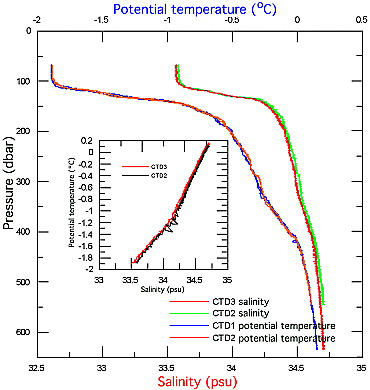
\includegraphics[width=0.7\textwidth]{chapters/4/oceanobs3.png}
\caption[Petermann observations]{Temperature and salinity profiles beneath a channel in the Petermann Glacier in Greenland \cite{rignot2008channelized}. A CTD instrument is measured the salinity, temperature, and pressure of water. 1 dbar = 1 meter of sea water.}
\label{fig:oceanobs3}
\end{figure}

Most descriptions of channel conditions are estimations from numerical model outputs.
Ice shelf channels have been modelled using a variety of ocean modelling techniques  \citep[e.g.][]{millgate2013effect,gladish2012ice,sergienko2013basal,payne2007numerical}. 
Some channel descriptions assume that a buoyant subglacial plume is the dominant process, so use a plume model to describe channel melt \citep[e.g.][]{gladish2012ice, sergienko2013basal}.
The majority of these descriptions are based on the formulation found in \cite{jenkins2011convection} and described in detail by \cite{hewitt2020subglacial}.
The \cite{jenkins2011convection} one dimensional plume model is based on conservation equations for mass, momentum, heat and salt, whereby melt rate is described in terms of plume thickness, speed, salinity, and temperature. This model forms the basis of sub--ice--shelf plume theory. Various configurations or scalings of the model can provide insights into plume behaviour. For example, if subglacial discharge is included in the model, the buoyancy flux driven by basal melt is negligible near the outlet. The one dimensional model has been used to approximate melt from subglacial outlet flux \cite[e.g.][]{gourmelen2017channelized} or outlet flux from melt rate (\cite[e.g.][]{marsh2016high}).

\cite{holland2006effects} extended this model to two horizontal dimensions, with depth--integrated conservation equations. In this model, the ocean is represented as a two-layer system consisting of a buoyancy-driven plume layer at the ice interface, which overlies a static  ambient layer with horizontally uniform stratification. This two layer system is typical of Greenlandic fjords \citep{hewitt2020subglacial}.
% buoyancy-driven ocean mixed-layer model 
Later, \cite{gladish2012ice,dallaston2015channelization} and \cite{sergienko2013regular} coupled the model to the Glimmer Community Ice-Sheet Model \citep{rutt2009glimmer} to model basal channel formation in the presence of an advecting ice shelf.
\cite{gladish2012ice} used the coupled models to describe the effect of basal channels on ice shelf melt rates. They imposed two wavelengths of cross-flow  roughness upstream of the grounding line to simulate topographic features. These features introduce grooves in the ice bottom that initiate melt channels downstream. \cite{gladish2012ice} suggest that ocean-induced melting, combined with rapid ice flow, deepened the existing channels and reproduced similar channelised basal morphology to that observed at the Petermann Glacier Ice Shelf in Greenland. In these model runs, introducing narrow channels suppressed melting at broader spatial scales, ultimately reducing the total amount of basal melt.
The same coupled ice--plume model was used by \cite{sergienko2013basal} to explore the conditions conducive to channel formation.  Their simulations suggest that channels form in response to melt water plume flow initiated at the grounding line if there are relatively high melt rates and if there is variability in ice shelf thickness transverse to ice flow.

Alternatively, \cite{millgate2013effect} used the full three dimensional Massachusetts Institute of Technology general circulation model (MITgcm, described in detail in Section \ref{sec:ocean_treatment}) to look at the impact of channels on melt rates on the Peterman Glacier tongue. They considered an idealised static ice shelf boundary and used an ice shelf basal mass balance package (\cite{losch2008modeling}, described in Section \ref{sec:ice_shelf_mb}) to approximate ice shelf melt. By running multiple model ice shelves with different numbers of channels, \citeauthor{millgate2013effect} found that having more channels reduced larger scale circulation which in turn reduced average melt rates under the glacier tongue.

To model ice shelf melt \cite{millgate2013effect} used an ice shelf basal mass balance package (`shelfice') developed by \cite{losch2008modeling}. This package has been used both to estimate ice shelf melt on real--world ice shelves \citep[e.g.][]{goldberg2019accurately}, and as a laboratory to better understand ice--ocean processes \citep[e.g.][]{xu2012numerical}. MITgcm functions on a large range of scales, for example, \cite{xu2012numerical} used high resolution grid cells of 20 m wide to model an ice shelf front, wheras \cite{naughten2021two} use grid cells up to 50 km to model the Filchner–Ronne Ice Shelf. 

A sensitivity analysis of MITgcm and `shelfice' found that the combination can successfully reproduce melt rates estimated using satellite altimetry \citep{goldberg2019accurately}. In this study, melt rates at the grounding zone were found to be highly sensitive, in particular to bathymetry. Accurate bathymetry was important for reproducing melt rates around the grounding zone because bathymetry impacted the transport of warm salty bottom water to the ice shelf. When comparing melt parametrisation, a velocity-independent melt model successfully reproduced the high melt rates observed near the grounding line, however, this parametrisation was believed to oversimplify melt when fast velocities were important, such as strong channelisation or subglacial discharge.

% Similarly, \cite{schodlok2012sensitivity} used MITgcm with the `shelfice' package to examine the ocean's role in the mass loss and grounding line retreat of Pine Island Glacier. They also concluded that accurate bathymetry is crucial to calculating melt rates at the grounding zone.

\cite{carroll2017subglacial} used MITgcm to model a fresh water plume driven by subglacial discharge in a fjord.  Similar to a sub--ice--shelf channel, this featured a laterally confined domain and estuarine flow with tides simulated by imposing an oscillating velocity on the open ocean boundary. \cite{carroll2017subglacial} find that in wider fjords ($\approx$ 10 km) circulation cells develop which increase the residence time of subglacial outlet water. 

% \subsection{ Goal}
% While existing channel models describe plume we have a gap that channel melting hasnt be modelled in the absence of advection.
In this chapter, we aim to better understand and constrain ocean processes in a basal channel at the grounding zone of the Kamb Ice Stream, using an ocean model to extrapolate from the existing knowledge of the channel shape and channel melt (described in Chapter \ref{ch:data}), and nearby oceanographic observations (described in Section \ref{sec:conditions}).  Firstly, we aim to better constrain subglacial discharge, which we assume causes the formation of the channel (Chapter \ref{ch:data}). Secondly, we aim to better describe meltwater plume dynamics by modelling melt without first assuming that a plume is driving melt. Lastly, we aim to understand how the channel is interacting with the  ocean, constraining the connection between the channel cavity and the larger Ross Ice Shelf cavity. 

To address these goals, we use MITgcm to model a channel with a domain shape based on its surveyed bathymetry (described in Chapter \ref{ch:data}). 
Ice-ocean interaction is modelled with the `shelfice' package, whereby the ice boundary is considered static. We run seven experiments using different boundary conditions (Section \ref{sec:model_runs}), as well as an eighth experiment which uses a contrived domain shape and has an ice shelf boundary which is adaptive in time.


In this chapter, we start by describing the domain shape used to model the surveyed channel  (Section \ref{sec:domain}). We next describe the different model setups (Section \ref{sec:model_runs}), before explaining the MITgcm set up, and its treatment of the ocean (Section \ref{sec:ocean_treatment} and ice shelf (Section \ref{sec:ice_shelf_mb}). We outline the process followed to model active melt in the adaptive domain (Section  \ref{sec:ablation_iterator}) Next, we describe the model outputs one by one: `Control' (Section \ref{sec:control_run}), `Weak inflow' (Section \ref{sec:weak_BC_results}), `Medium inflow' (Section \ref{sec:medium_inflow}), `Surge inflow' (Section \ref{sec:surge_inflow}), `More ocean connection' (Section \ref{sec:fresh_output}), `Fast inflow' (Section \ref{sec:high_velocity}), and `Adaptive domain' (Section \ref{sec:adaptive_dom_results}).
In these model runs, our initial and boundary conditions are based on direct oceanographic observations of the ice shelf cavity nearby.

\section{Study area} \label{sec:conditions}

\begin{figure}[!ht]
\centering
    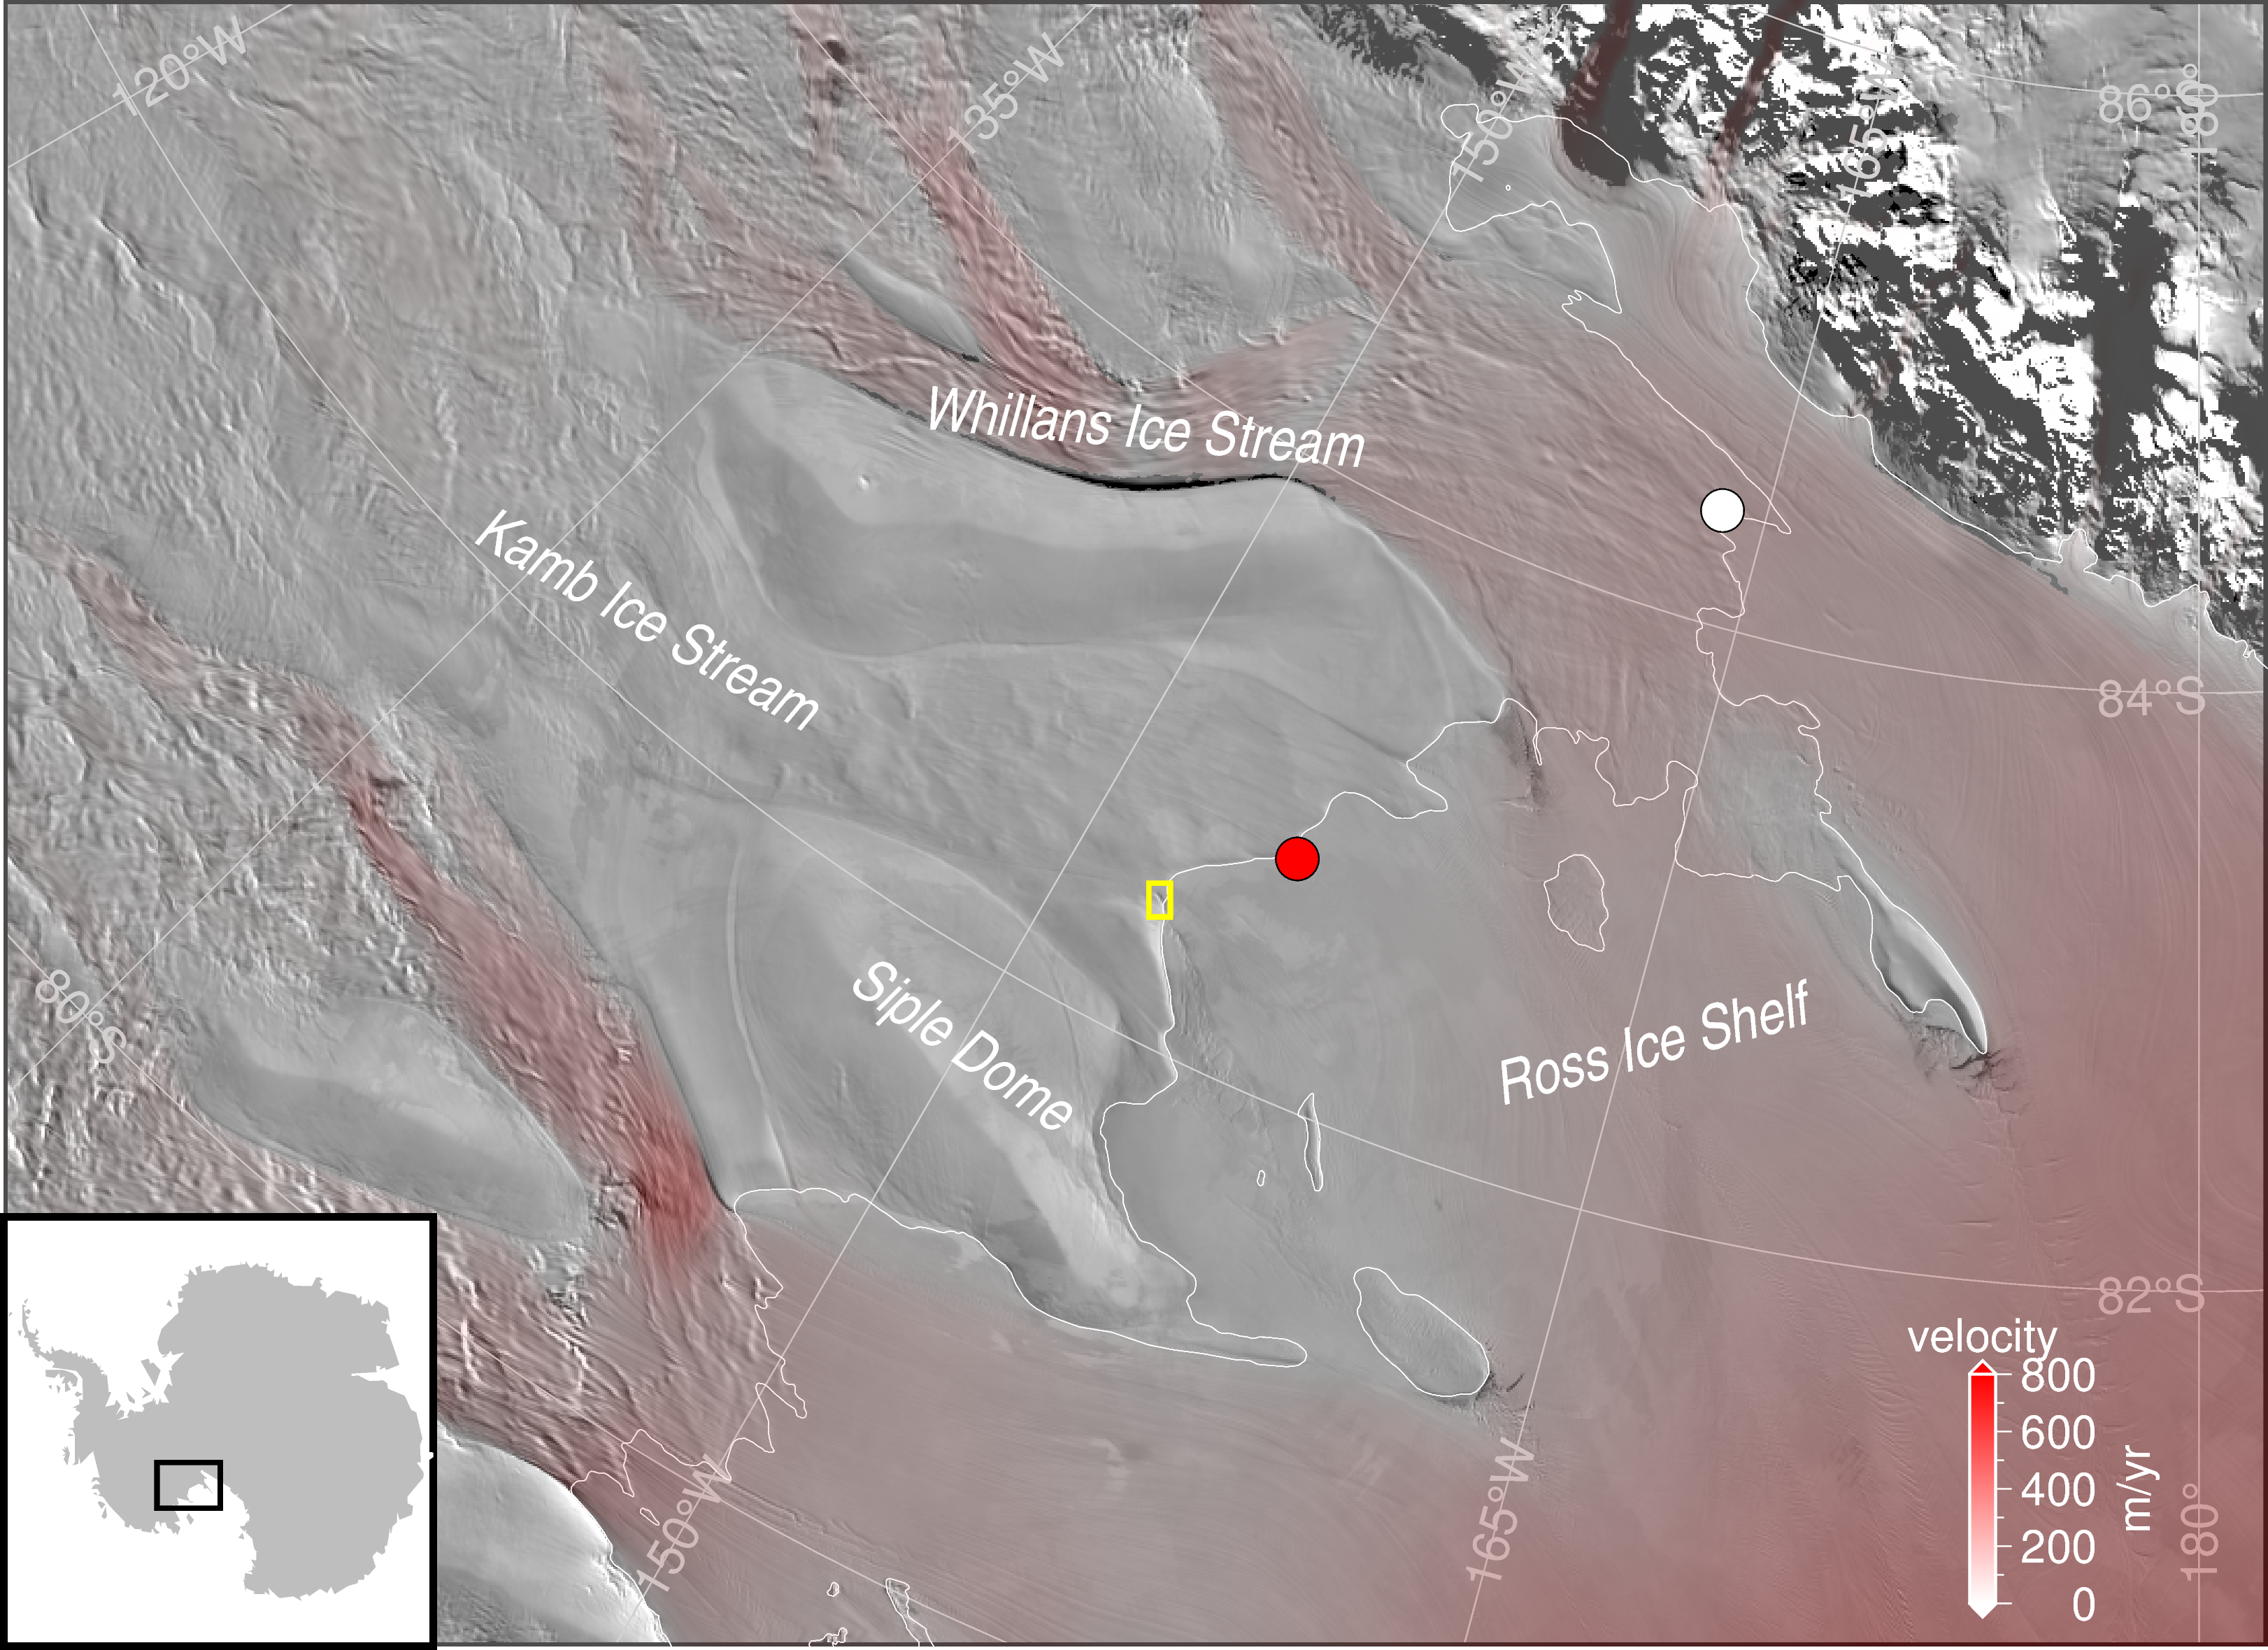
\includegraphics[width=1\textwidth]{chapters/4/drilling_locations_small.png}
    \caption[Drilling locations]{Locations of direct access near the grounding line of the Siple Coast. Drilling at `KIS1' shown by red circle (Figure \ref{fig:oceanobs2}). Drilling at Whillans Ice Stream shown by white circle (Figure \ref{fig:oceanobs1}). Yellow square outlines channel and future drilling location.}
    \label{fig:map_drill}
\end{figure}

\begin{figure}[!ht]
\centering
    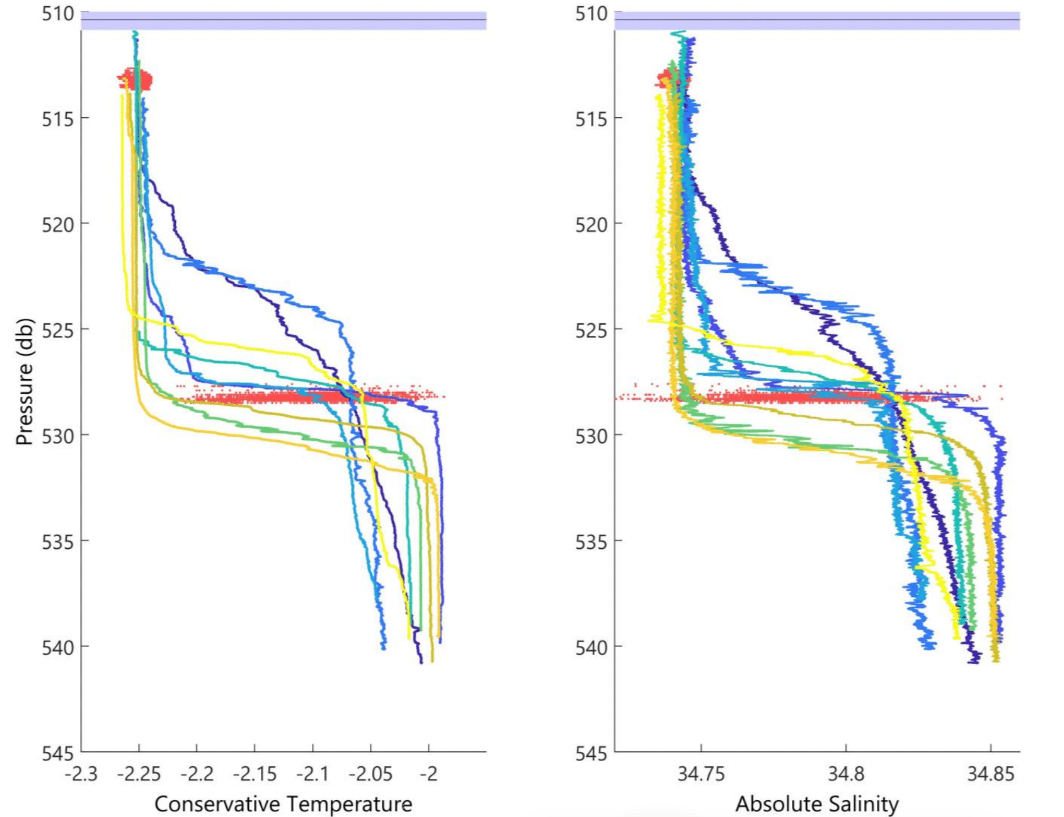
\includegraphics[width=1\textwidth]{chapters/4/oceanobs2.jpg}
    \caption[KIS1 observations]{Figure from \cite{robinson2020ice} showing temperature and salinity profiles beneath the Ross Ice Shelf at `KIS1', 50 km from the channel study location. Different colors show profiles from different times over a two week long period. Location of direct access shown in Figure \ref{fig:map_drill} as a red circle.}
    \label{fig:oceanobs2}
\end{figure}

\begin{figure}[!ht]
\centering
    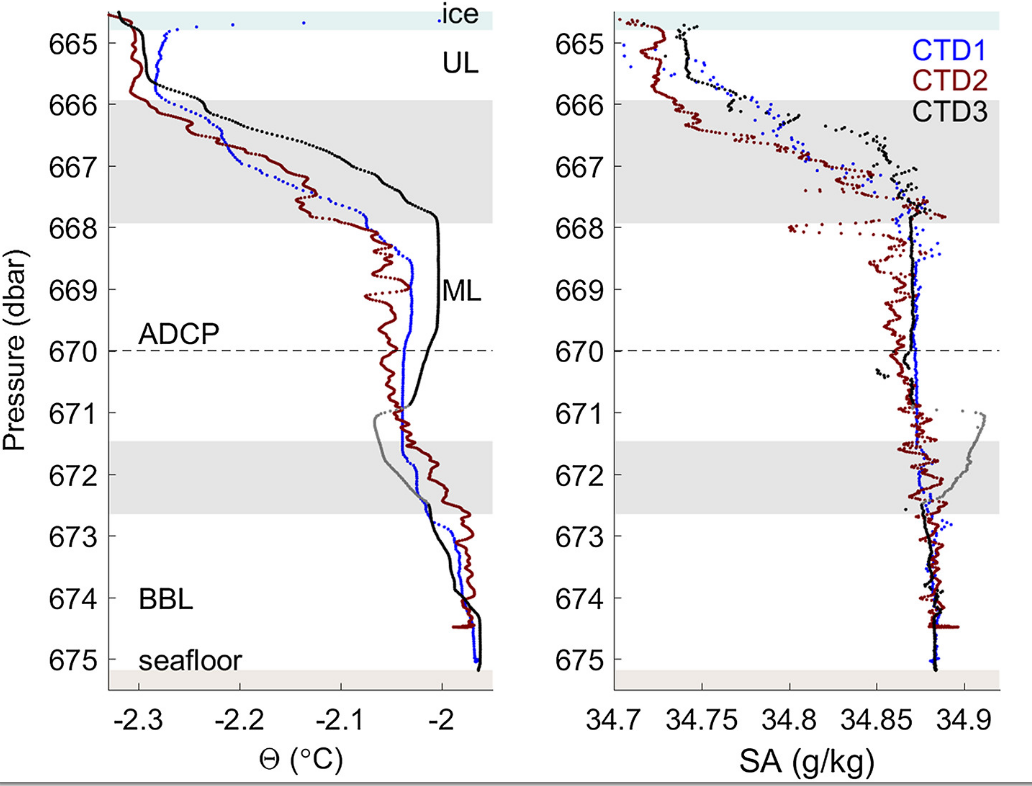
\includegraphics[width=1\textwidth]{chapters/4/oceanobs1.png}
    \caption[Whillans observations]{Figure from \cite{begeman2018ocean} shows temperature ($\theta$) and salinity (SA) profiles beneath the Ross Ice Shelf at the grounding zone of the Whillans Ice Stream. Location of direct access shown in Figure \ref{fig:map_drill} as a white circle.}
    \label{fig:oceanobs1}
\end{figure}

Here, we present a study of ice--ocean interaction in a basal channel at the grounding zone of the Kamb Ice Stream (location in Figure \ref{fig:map_drill}). 
The channel extends 6 km upstream of the previously estimated grounding line of the stagnant Kamb Ice Stream, and incises up to 50 \% of the ice thickness. The channel is manifest on the ice surface as a  10,000 x 3000 x 20 m valley, and is visible from the ground and in satellite imagery. Because the channel sits at the outlet of estimated subglacial drainage paths (Chapter \ref{ch:data}), the channel is likely formed by a buoyant meltwater plume triggered by subglacial discharge \citep{kim2016active, alley2016impacts}.

While there are no observations of ocean conditions in the channel beneath the Kamb Ice Stream, two drilling campaigns have accessed the ocean cavity nearby. 
Fifty kilometres away from the channel at the field camp, `KIS1' oceanographic instruments were deployed through a hole drilled through the 580 m thick ice shelf in 2019-20 \citep{robinson2020ice}. The 30 m deep water column had two distinct layers (Figure \ref{fig:oceanobs2}). The top 18 m had temperature and salinity of 34.75 g/kg and -2.25 \textdegree C (Figure \ref{fig:oceanobs2}). The bottom 12 m had a temperature and salinity of -2.0 and 34.84 g/kg.
250 km along the coastline, \cite{begeman2018ocean} accessed the 10 m deep ocean cavity at the Whillans Ice Shelf. Similarly, salinity and temperature profiles (Figure \ref{fig:oceanobs1}) show two distinct layers. A 2 m deep fresh, cool layer with salinity and temperature of 34.73 g/kg and -2.3 \textdegree C was found above a layer with salinity and temperature of 34.87 g/kg and -2.0 \textdegree C.
% Various model outputs  products cover the area, \cite[e.g.][]{holland2003modelling}. The grid cells are so large theae just as far away as the KIS1 observations.
While these observations inform the set up of the model runs, melt rate and subglacial discharge estimates inform the model interpretation.
In Chapter \ref{ch:data}, we estimated melt rates to be more than 20 m/yr over a 200 m x 1.5 km basal area at the head of the channel. Three and a half kilometres downstream, we found we found accretion across the channel, peaking at the channel apex, and melt on either side of the channel profile. Nearby at Whillians Ice Stream, \cite{marsh2016high} found melt of 22.2 $\pm$ 0.2 m/yr in a channel. Lastly, subglacial discharge from above grounding line was estimated by \cite{le2009subglacial} to be $23.9 \mathrm{m}^3/\mathrm{s}$.


\section{Method}

% see phd thesis https://eprints.soton.ac.uk/424757/1/Burns_Helen_June_2018_Thesis_corrections.pdf
% https://eprints.soton.ac.uk/447348/1/Bett_David_Thesis_final_Feb21.pdf
\subsection{The prescribed domain} \label{sec:domain}


\begin{figure}[!ht]
\centering
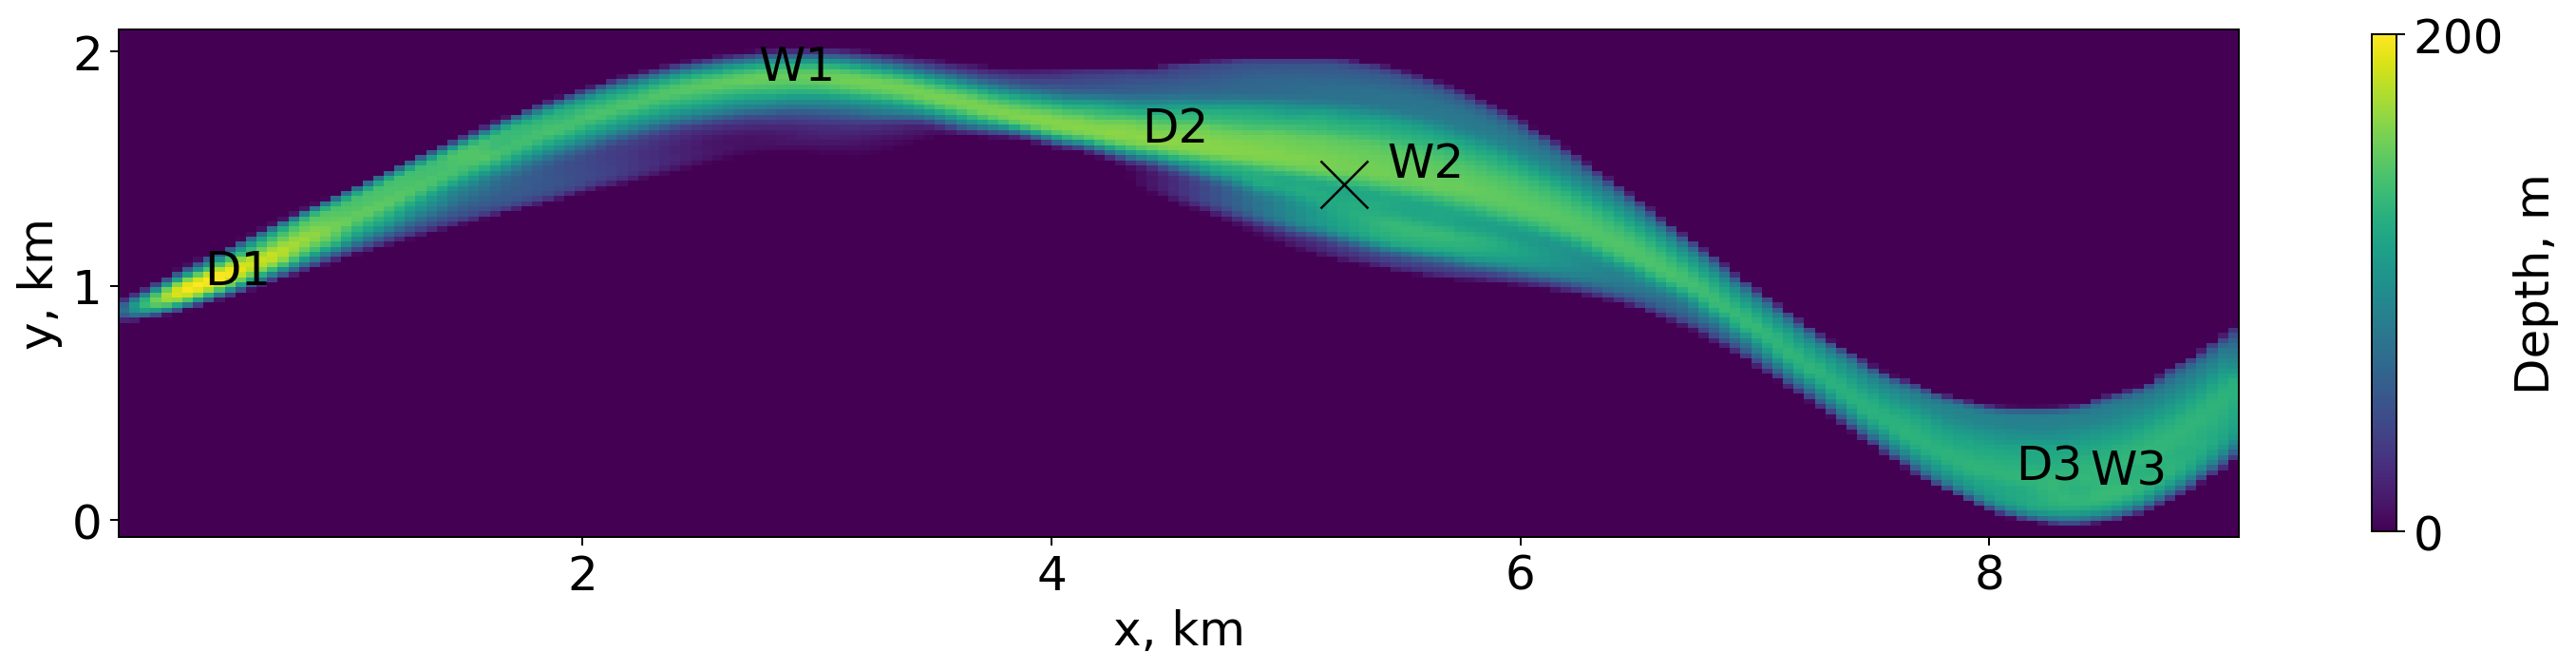
\includegraphics[width=1\textwidth]{chapters/4/domain.png}
\caption[Domain]{Domain shape used in model experiments. An ocean cavity bounded by ice spans 9.2 km between the upstream and downstream boundaries. W1-W3 are locally wide areas of the channel and D1-D3 are locally deep areas of the channel. X is the location of profiles shown Figures \ref{fig:weak_inflow_TSU} and \ref{fig:compare_all_TSU} }
\label{fig:domain}
\end{figure}

To investigate water circulation in the subglacial channel we considered a model domain based on the interpolated ice base map (Section \ref{sec:icebasetopog}), simplified for the constraints of a numerical ocean model. 
To construct the model domain, all radar lines crossing the channel were resampled spatially from the channel apex to both sides of the channel. Equivalent points from each line were then interpolated downstream with a weighted B--spline. The upstream--most cross channel line was weighted 1 to constrain the channel inception then downstream points were weighted 0.1. This gave a smoother ice base map than that described in Section \ref{sec:icebasetopog}, with a standard deviation of the error in the vertical direction of 10 m.  Additionally, the B--spline was smoothed such that $ \Sigma ((w  (z - g))^2) <= 50 $ where x is distance downstream, w is the weight given to a point, $z$ is height and $g(x)$ is the smoothed interpolation of $(x,z)$.
The interpolated channel area was then spliced onto a flat plane at the level of mean ice base elevation, representing the model ground. The resulting shape was then rotated, and interpolated using nearest neighbours onto a regular grid so that the x direction was down channel and y direction was across the channel. Lastly, the shape was smoothed with an order zero convolution with a Gaussian kernel, with a standard deviation for the Gaussian kernel of 1. A smoother shaped cavity is easier to solve computationally.
The upstream opening and dowstream end of the channel were cropped by 8 m and 4 m respectively to create larger open boundaries. 
The domain was represented on a cartesian grid with (x, y, z) resolution of (200, 100, 136 m). Cells edges measure (45.4, 21.8, 4.0 m)  respectively.

\begin{figure}[!ht]
\centering
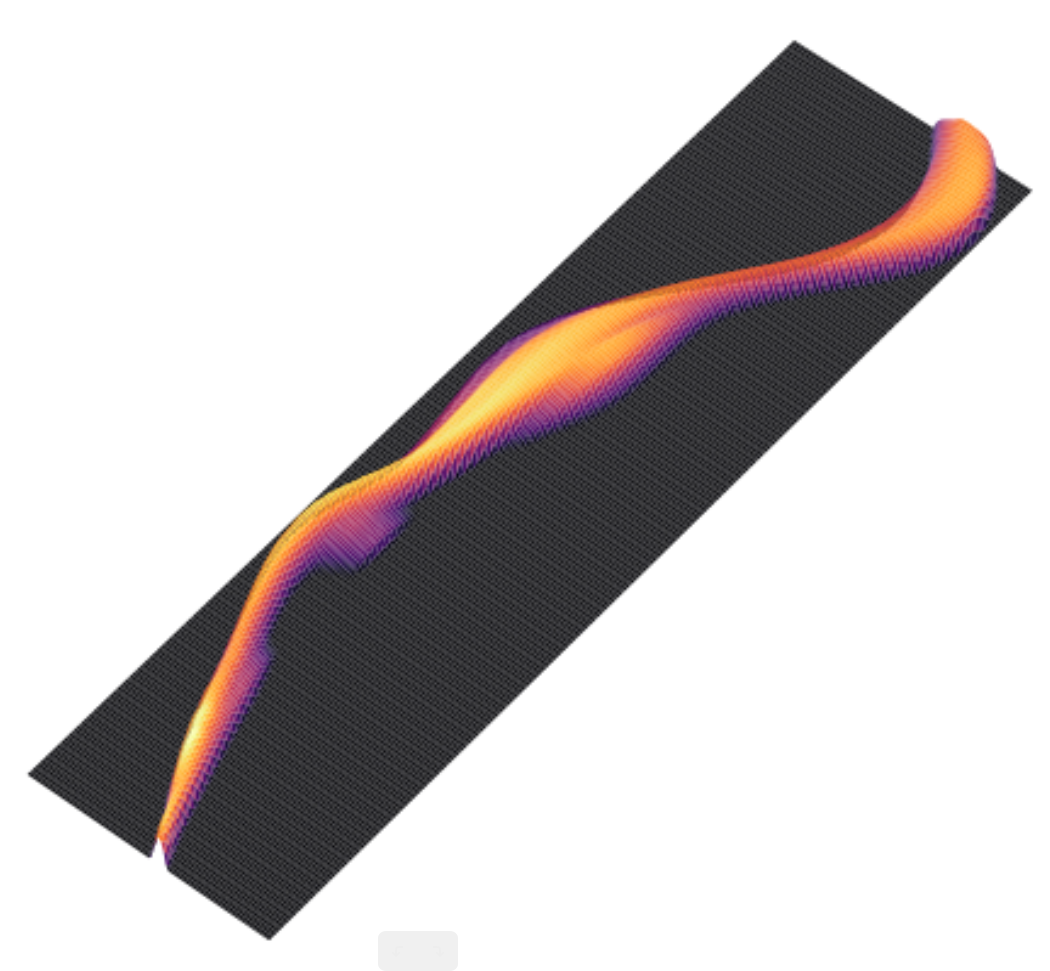
\includegraphics[width=0.8\textwidth]{chapters/4/3d_domain.png}
\caption[3D domain]{To scale, 3D depiction of the domain shown in Figure \ref{fig:domain}. }
\label{fig:3d_domain}
\end{figure}

The resulting domain is 9.2 km long and 2.1 km wide (Figure \ref{fig:domain} and \ref{fig:3d_domain}). The sea--water filled channel is bounded by ice on its walls and roof, and an ice--free sea floor -675 m below sea level. The open upstream boundary is designed to represent subglacial discharge entering the channel, and the open downstream boundary represents the connection with the ocean. In this chapter, we use the terms upstream, downstream, true left, and true right for describing horizontal locations in the ocean cavity. 
% These correspond to the planes x=0 km, x= 9 km, y = 2 km and y =0 km respectively.
The terms top and bottom refer exclusively to vertical position in the water column.
% , to -380 m and -540 m respectively. 

Following down the apex of the channel, the ice roof of the cavity has local maxima in thickness of the water column of 200, 165 and 135 m at $x=$ 0.55, 4.5, and 8.7 km which we name D1, D2 and D3 respectively (Figure \ref{fig:domain}). The channel is narrowest (130 m wide) at the upstream boundary. Downstream, the channel features three wide areas we name W1, W2, and W3 which are 460, 900, and 525 m wide at $x =$ 2.9, 5.6, 8.6 km respectively (Figure \ref{fig:domain}). These wide areas correspond with bends in the channel. Between wide sections the channel narrows to around 300-350 m. 


For each model run, the upstream boundary was prescribed with a constant temperature, salinity and velocity. At the downstream boundary temperature (T), salinity (S) and the x--component of velocity (U) were prescribed with a logarithmic profile dependent only on height. This was calculated as a logspace which spans from the bottom to top of the downstream boundary (labelled $V^d_B$ and $V^d_T $ ) along the height of the boundary, as follows, where $V \in \{T,S,U\}$,
\[
    \left(V^d_B \dots V^d_T \right)= 
\begin{cases}
    10^{(log_{10}|v_0|...log_{10}|v_n|} + V^d_B - v_0, & \text{if } V^d_T - V^d_B>0\\
    -10^{(log_{10}|v_0|...log_{10}|v_n|)} + V^d_B - v_0,              & \text{if }   V^d_T - V^d_B<0,
\end{cases}
\]

and all operations are element--wise. The vector $(v_0...v_n)$ is linearly increasing, and spans $v_0$ to $v_n$ where $ v_n = V^d_B - V^d_T-v_0$ and $v_0 \ll 1$. The parameter $v_0$ is used to tune the gradient of the profile, and $n-1$ is the numer of cells which span the open boundary.
Values $\left(T^d_B, T^d_T\right)$, $\left(S^d_B, S^d_T\right)$ and $U^d_T$  were prescribed, then  $U^d_B$ was calculated so that flux out of the downstream boundary is equal to that flowing in through the upstream boundary.
The area of the upstream boundary of the model domain is 5270 $\mathrm{m}^2$. Boundary velocities of 0.0004, 0.01 and 0.1 $\mathrm{m}$/s correspond to flow rates of 2.1 $\mathrm{m}^3$/s, 52.6 and 526 $\mathrm{m}^3$/s respectively. 

\subsection{Model run descriptions} \label{sec:model_runs}

The model was run with 5 second time steps, and was first spun up for 55 days with the run `Control'. The run `Control' had no prescribed flux, temperature or salinity at the boundary (it has Neumann boundary conditions), and an initial temperature and salinity of  -2.0$^{\circ}$C  and 34.73 g/kg. All other model runs had initial conditions from `Control' at 55 days, except `Fast inflow' which had initial conditions from `More ocean connection' at 8 days, and `Adaptive domain' which is described in Section \ref{sec:ablation_iterator}.

The model was run with different boundary conditions described in Section \ref{tab:model_runs}. The downstream boundary replicates ocean conditions from the Ross Ice Shelf cavity, with values taken from sub--ice--shelf observations made nearby by \citep{robinson2020ice}. 
Temperature at the bottom and top of the downstream boundary are set to -2.0 \textdegree C and -2.25 \textdegree C and salinity at the bottom and top are set to 34.75 g/kg and 34.64 g/kg respectively. 
The upstream boundary simulates subglacial discharge, which is likely fresh or at least relatively fresh depending on how far upstream ocean water mixes with the discharge. The model run `Fresh inflow' and `Adaptive domain' have discharge with no salinity and at the pressure melting point. With these conditions the model cannot numerically converge with more than 0.4 mm/s velocity inflow at the upstream boundary. Most model runs have temperature and salinity of -1.213 \textdegree C and 16.46 g/kg which are halfway between the bottom water conditions of -2.0 \textdegree C, 34.75 g/kg and the pressure melting point. This represents a partially mixed subglacial discharge. Because its not fully fresh we can run the model with much higher velocities without the model failing. The model run `Fast inflow' has a upstream boundary 3/4 of the way towards the pressure melting point from -2.0 \textdegree C, 34.75 g/kg. `More ocean connection' and `Fast inflow' have fresher output water on the downstream boundary on the ice-ocean boundary. 
\begin{table}[!ht]
\begin{tabular}{|c|c|c|c|c|c|c|c|}
    \hline
    & $T^{u}$ & $S^{u} $ & $U^{u}$& $T^d_T$ & $S^d_T$ & $U^d_T$ & $v_0$ \\
     \hline
    Control & -- & -- & --& -- &--  &--  &--  \\
    % \hline
    Weak inflow & -1.213 & 16.46  &0.0004 &  -2.25 & 34.64 & 0.04 & $10^{-8}$  \\
    % \hline
    Fresh inflow & -0.51 & 0.0 &0.0004 &  -2.25 & 34.64 & 0.04 & $10^{-8}$  \\
    % \hline
    Medium inflow & -1.213 & 16.46 & 0.01 &  -2.25 & 34.64 & 0.04  & $10^{-8}$ \\
    % \hline
    Surge inflow --- pre/post--surge  & -1.213 & 16.46  &0.0004 &  -2.25 & 34.64 & 0.04 & $10^{-8}$ \\
    % \hline
    Surge inflow --- surge & -1.213 & 16.46 & 0.01 &  -2.25 & 34.64 & 0.04  & $10^{-8}$ \\
    % \hline
    More ocean connection & -1.213 & 16.46 & 0.01 &  -1.21 & 16.46 & 0.04& $10^{-4}$  \\
    % \hline
    Fast inflow & -1.61 & 25.6 & 0.1 & -0.82 & 7.3  & 0.1 & $10^{-4}$ \\
    \hline
    Adaptive domain  & -0.51 & 0.0 &0.0004 &  -2.25 & 34.64 & 0.04 & $10^{-8}$ \\
    \hline
\end{tabular}
\caption[Model run parameters]{\label{tab:model_runs} Subscript $^u$ and $^d$ denote upstream and downstream boundaries respectively. Superscript $_T$ denotes top of the water column. (T,S,U) have units of (\textdegree C,g/kg, m/s)  }
\end{table}

\subsection{Model description}
\subsubsection{Ocean treatment} \label{sec:ocean_treatment}

The MIT general circulation model (MITgcm) \citep{marshall1997finite,marshall1997hydrostatic} is used to model the ocean and its interaction with the ice shelf in the ice bounded cavity. MITgcm is equipped to model metre length scale processes like turbulence and convection \citep[e.g.]{xu2012numerical}.
% This section describes the ocean modelling. Section \ref{sec:ice_shelf_mb} focuses on the treatment of ice--ocean interactions.
Because we are interested in sub-kilometre length scales we use a non-hydrostatic configuration with a free surface. Our configuration of MITgcm is based on ISOMIP experiments (Ice-Shelf Ocean Model Intercomparison Project) \citep{holland2003ice}.  In each model timestep, MITgcm algorithms solve the Boussinesq form of the Navier Stokes equations for an incompressible fluid, with a spatial finite-volume discretization on a cartesian grid.
The Boussinesq equations can be written as,


Conservation of momentum
\begin{align}
    \frac{\partial \mathbf{v_h}}{\partial t}  &= \mathbf{G_{v_h}} -  \nabla_h p \label{eq:momentum}\\
    \frac{\partial w}{\partial t} &= \mathbf{G_w} - \frac{\partial p }{\partial z} \label{eq:momentum2}
\end{align}
Continuity
\begin{align}
    \nabla \cdot \mathbf{v} &= 0 \label{eq:continuity}
\end{align}
Heat
\begin{align}
    \frac{\partial T}{\partial} &= G_T
\end{align}
Salt
\begin{align}
    \frac{\partial S}{\partial} &= G_S 
\end{align}
Equation of state
\begin{align}
    \rho &= \rho(T,S, p),
\end{align}
% \begin{align}
%     \rho_0 D_t \mathbf{v} + 2 \Omega \times \rho_0 \mathbf{v} + g \rho \hat{k} + \nabla p &= \mathbf{F} \label{eq:momentum}\\
%     \delta_t \eta + \nabla \cdot (H + \eta ) \mathbf{v} &= P - E \label{eq:momentum2}\\
%     \rho_0 \nabla \cdot \mathbf{v} &= 0 \label{eq:continuity}\\
%     D_t \theta &= Q_{\theta}\\
%     D_t S &= Q_S \\
%     \rho &= \rho(S,\theta, p),
% \end{align}
Where the $(x,y,z)$ components of velocity are  $\mathbf{v}$ are  $(u,v,w) = (\mathbf{v_h},w) $, and $\mathbf{G_v} = (G_u,G_v,G_w)$ and $(G_S,G_T)$ represent inertial, Coriolis, metric, gravitational and forcing terms. Pressure, from resting sea-level is $p$, $T$ is potential temperature, $S$ is salinity.
These equations are solved on an Arakawa C--grid in the horizontal direction (Figure \ref{fig:c_grid}), and a Lorentz grid in the vertical \citep{adcroft1997representation}. This leads to a tidy discretization of the incompressible continuity equation (Equation \ref{eq:continuity}),

\begin{figure}[!ht]
\centering
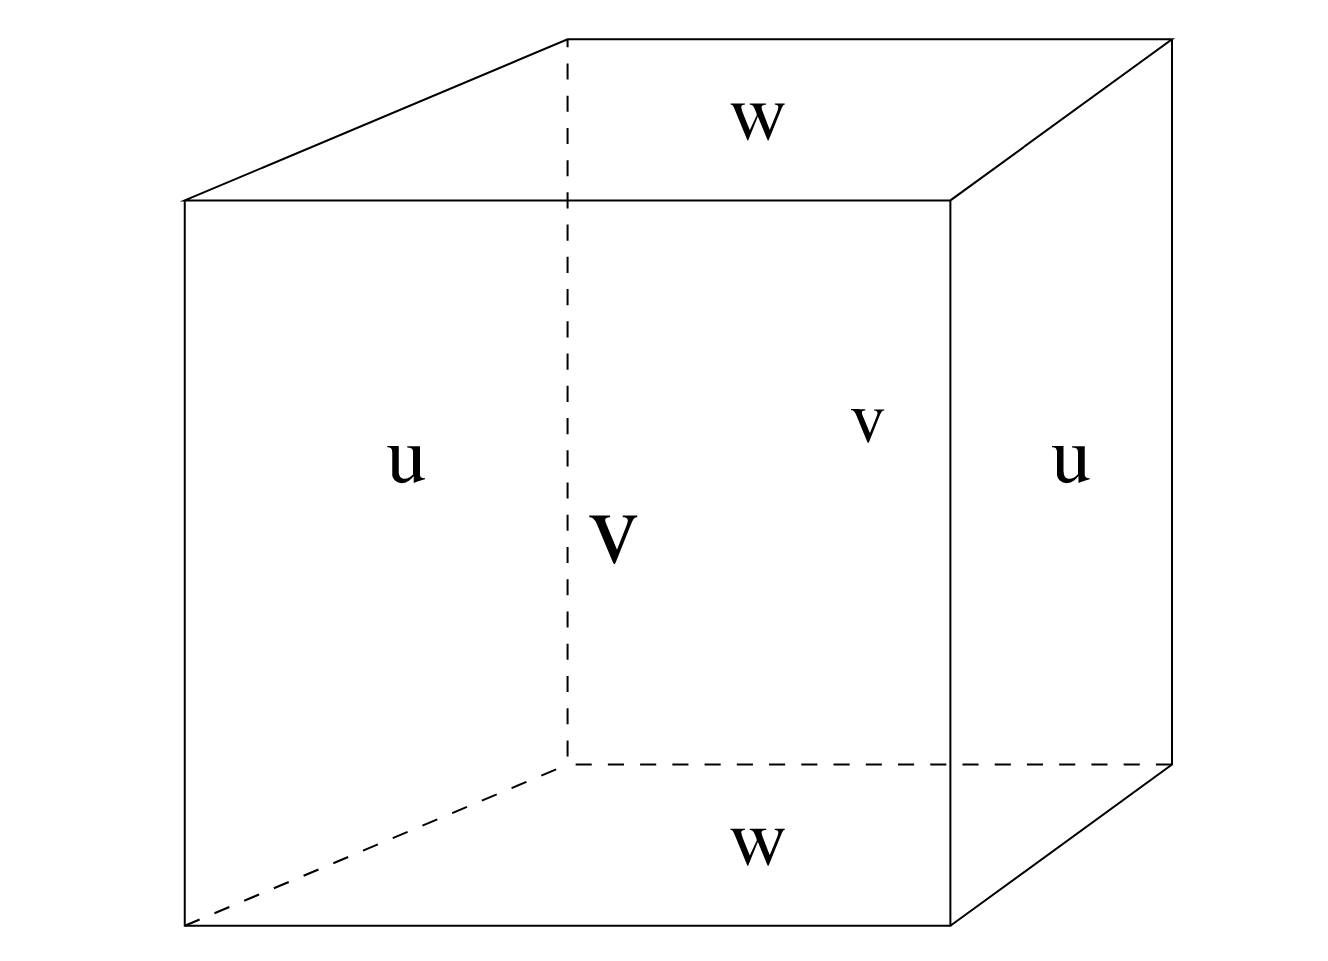
\includegraphics[width=0.4\textwidth]{chapters/4/c_grid.png}
\caption[C--grid]{ Three dimensional staggering of velocity components. $(u, v, w)$ are the $(x,y,z)$ components of velocity respectively. Each component of velocity is calculated on the cell boundary normal to the component direction. This facilitates the natural discretization of the continuity and tracer equations.}
\label{fig:c_grid}
\end{figure}

\begin{align}
    A^u_{east} u_{east} - A^u_{west} u_{west}+A^v_{north} v_{north}-A^v_{south} v_{south}+A^w_{up} w_{up}-A^w_{down} u_{down} = 0
\end{align}

where $A_{heading}$ are the cell faces and $(u, v, w)$ are the $(x,y,z)$ components of $\mathbf{v}$. The horizontal momentum equation is solved with the projection method (operator splitting), in which the discretized equation  (Equation \ref{eq:momentum}) solves the pressure forces and viscous forces separately in two half steps. 
\begin{align}
    {\frac  {{\mathbf  {v}}^{*}-{\mathbf  {v}}^{n}}{\Delta t}}&= G_{v_h}  \label{eq:first_half}\\
    {\mathbf  {v}}^{{n+1}}&={\mathbf  {v}}^{*}-{\Delta t}\,\nabla p^{{n+1}} \label{eq:second_half}
\end{align}

% -({\mathbf  {u}}^{n}\cdot \nabla ){\mathbf  {u}}^{n}+\nu \nabla ^{2}{\mathbf  {u}}^{n}
In the first half step (Equation \ref{eq:first_half}), steps velocity $\mathbf{v}$ forward to find an intermediate velocity $\mathbf{v}^{*}$ by ignoring the pressure gradient term. In the second half step (Equation \ref{eq:second_half}), the intermediate velocity is corrected to obtain the final solution of the time step ${ \mathbf {v} ^{n+1}}$.
Substituting the two momentum equations (Equation \ref{eq:momentum} and \ref{eq:momentum2}) into the depth integrated conservation of mass equation (\ref{eq:continuity}) results in an elliptic equation which is solved for pressure. The algorithms used in this process are outlined in \citep{marshall1997finite,marshall1997hydrostatic}. Next we outline the model treatment of ice--ocean interation.
% %######
% % Nonhydrostatic.  In  the nonhydrostatic model, all terms in the incompressible Navier Stokes equations (7)-(18) are retained. A three-dimensional elliptic equation (24) must be solved with boundary conditions (25). 

% % In the non--hydrostatic primitive equations (described in detail in \citep{marshall1997hydrostatic}) a three dimensional elliptic equation must be solved subject to Neumann boundary conditions (see below). It is important to note that use of the full NH does not admit any new ‘fast’ waves in to the system - the incompressible condition (1.3) has already filtered out acoustic modes. It does, however, ensure that the gravity waves are treated accurately with an exact dispersion relation. The NH set has a complete angular momentum principle and consistent energetics - see White and Bromley (1995) [WB95]; Marshall et al. (1997a) [MHPA97].

%  To do this we must split the density thus:
% $$\rho  = \rho_0 + \rho'$$

% We then assert that variations with depth of 
%  are unimportant while the compressible effects in 
%  are:
% $$\rho_0 = \rho_c$$
% $$\rho'  = \rho(\theta,S,p_0(z)) - \rho_0$$

% DO INCOMPRESSIBLE
% % https://extranet.gfdl.noaa.gov/~aja/papers/ECMWF2004-Adcroft.pdf
% % https://mitgcm.readthedocs.io/en/latest/overview/eqn_motion_ocn.html

% where v is velocity, $p$ is pressure $\rho$ is density, $\eta$ is the displacement of free surface
% from resting sea-level, $\theta$ is potential temperature, $s$ is salinity, $\rho_0$ is the reference
% density, $g$ is gravitational acceleration, $H$ is bottom depth.
% Note that the hydrostatic pressure of the resting fluid, including that associated with $\rho_c$, is subtracted out since it has no effect on the dynamics.
% Though necessary, the assumptions that go into these equations are messy since we essentially assume a different EOS for the reference density and the perturbation density. Nevertheless, it is the hydrostatic ($\epsilon_{nh} = 0$) form of these equations that are used throughout the ocean modeling community and referred to as the primitive equations (HPE’s).

% finite volume methodology (Adcroft et al., 1997), where the governing equations are integrated over
% finite volumes and applying the Gauss-divergence theorem to give a continuity in
% the form:

% Discretisation, vertical grid and partially filled grid cells.

% 

% Figure 2.7 shows the components of flow (u,v,w) staggered in space such that the zonal component falls on the interface between continuity cells in the zonal direction. Similarly for the meridional and vertical directions. The continuity cell is synonymous with tracer cells (they are one and the same).
% \begin{align}
%     A^u_{east} u_{east} - A^u_{west} u_{west}+ A^v_{north} v_{north} - A^V_{south} v_{south} + A^w_{up}w_{up} -A^w_{down}w_{down} = 0
% \end{align}
% written in terms of the normal flow (u, v, w) across cell faces A direction. With no
% normal flow at rigid boundaries (volume flux though a rigid boundary is set to
% zero) (see Fig. 1.4). The components of velocity are staggered on an Arakawa C
% grid (Chang et al., 1977) in the horizontal and a Lorenz grid in the vertical (Lorenz ,
% 1960) - see Fig. 1.5.


% from docs
% The basic algorithm employed for stepping forward the momentum equations is based on retaining non-divergence of the flow at all times. This is most naturally done if the components of flow are staggered in space in the form of an Arakawa C grid (Arakawa and Lamb, 1977 [AL77]).
% The non-dimensional fractions (or h-facs as we call them) are calculated from the model depth array and then processed to avoid tiny volumes. The rule is that if a fraction is less than hFacMin then it is rounded to the nearer of  or hFacMin or if the physical thickness is less than hFacMinDr then it is similarly rounded. The larger of the two methods is used when there is a conflict. By setting hFacMinDr equal to or larger than the thinnest nominal layers, 
% , but setting hFacMin to some small fraction then the model will only lop thick layers but retain stability based on the thinnest unlopped thickness; 
% .

\subsubsection{Ice shelf treatment} \label{sec:ice_shelf_mb}

Ablation and accretion at the ice--ocean interface were paramerized by the MITgcm `shelfice' package described in \citep{losch2008modeling}. This assumes that the ice shelf is stable and floating. `Shelfice' solves the following three equations from \cite{hellmer1989two}, describing the conservation of heat, the conservation of salt, and temperature as a linear function of salinity respectively.

\begin{align}
    \rho_0 c_0 \gamma_T ( T - T_b) = m \rho_0 L + \rho_1 c_1 \kappa_1 \left( \frac{T_b - T_I}{H_I} \right), \label{eq:melt}\\
    \gamma_S \left( S- S_b \right) = m S_b, \\
    T_b = a S_b + b + c d,
\end{align}
where $m$ is basal melt rate (mass balance), $H_I$ is ice-shelf thickness, and $T_b$ and $S_b$ are temperature and salinity at the ice-ocean interface, $d$ is ice draft, and $\rho_o$ is density of the ocean surface layer, with constants outlined in Table \ref{tab:shelf_melt_params}. 
 
\begin{center}
\begin{tabular}{ c|c|c|c } 
\hline
 Specific heat capacity of water & $c_o$  & 53994  &  J/ kg \textdegree C \\
 Specific heat capacity of ice & $c_I $ & 52000 &  J/ kg\textdegree C  \\
 Latent heat of ice fusion & $L$ & $3.34\times 10^5$ & J/ kg \\
 Density of the ice shelf &$\rho_I$& $917 $ & $kg/ m^3$ \\
 Molecular thermal conductivity of the ice shelf & $\kappa_I $ & $ 1.541 \times 10^{-6}$ & $\text{m}^2/\text{s}$ \\
 Core temperature of the ice shelf & $T_I$& $-20$ & \textdegree C\\
 Linear freezing equation coefficients  & $a$ &  $0.0575$ & \textdegree C/psu \\
 Linear freezing equation coefficients  & $b$ & $0.0901$ & \textdegree C \\
 Linear freezing equation coefficients &$c$& $7.61\times10^{-4}$ & \textdegree C / Pa \\
 Vertical eddy diffusivity & - & $5 \times 10^{-6}$ & $\mathrm{m}^2$s\\
 Vertical eddy viscosity & - & $1 \times 10^{-4}$ & $\mathrm{m}^2$/s\\
 Coriolis parameter & $f0$ & $ -1.446 \times 10^{-4}$ & $\mathrm{s}^{-1}$\\
 \hline
\end{tabular}
\label{tab:shelf_melt_params}
\end{center}



We used a velocity-dependent parameterization of thermal and haline transfer coefficients from \cite{holland1999modeling}:
\begin{align}
    \gamma_{T,S} = u_* \Gamma^f_{T,S}
\end{align}
where $u_* = \sqrt{c_d u^2_0}$ is the friction velocity, and $\gamma_{T}=0.011$, $\gamma_{S}=0.00031$ are the thermal and haline exchange velocities respectively. 
If the conduction of heat through the ice shelf is ignored, Equation \ref{eq:melt} shows that the melt rate $m$ can be solved as a product of the friction velocity, $u_*$ and thermal driving $(T - T_b)$ \citep{holland2008response}. Basal melt rate is calculated from the ocean properties in the cell vertically beneath an ice cell (Figure \ref{fig:melt_cells}). This takes the mean temperature and salinity from all cells within a distance dz (4 m) from the ice--ocean boundary, which could include a partial cell and a fraction of the full cell beneath it. In our configuration, partial cells with a minimum height of 30 cm were used.
\begin{figure}[!ht]
\centering
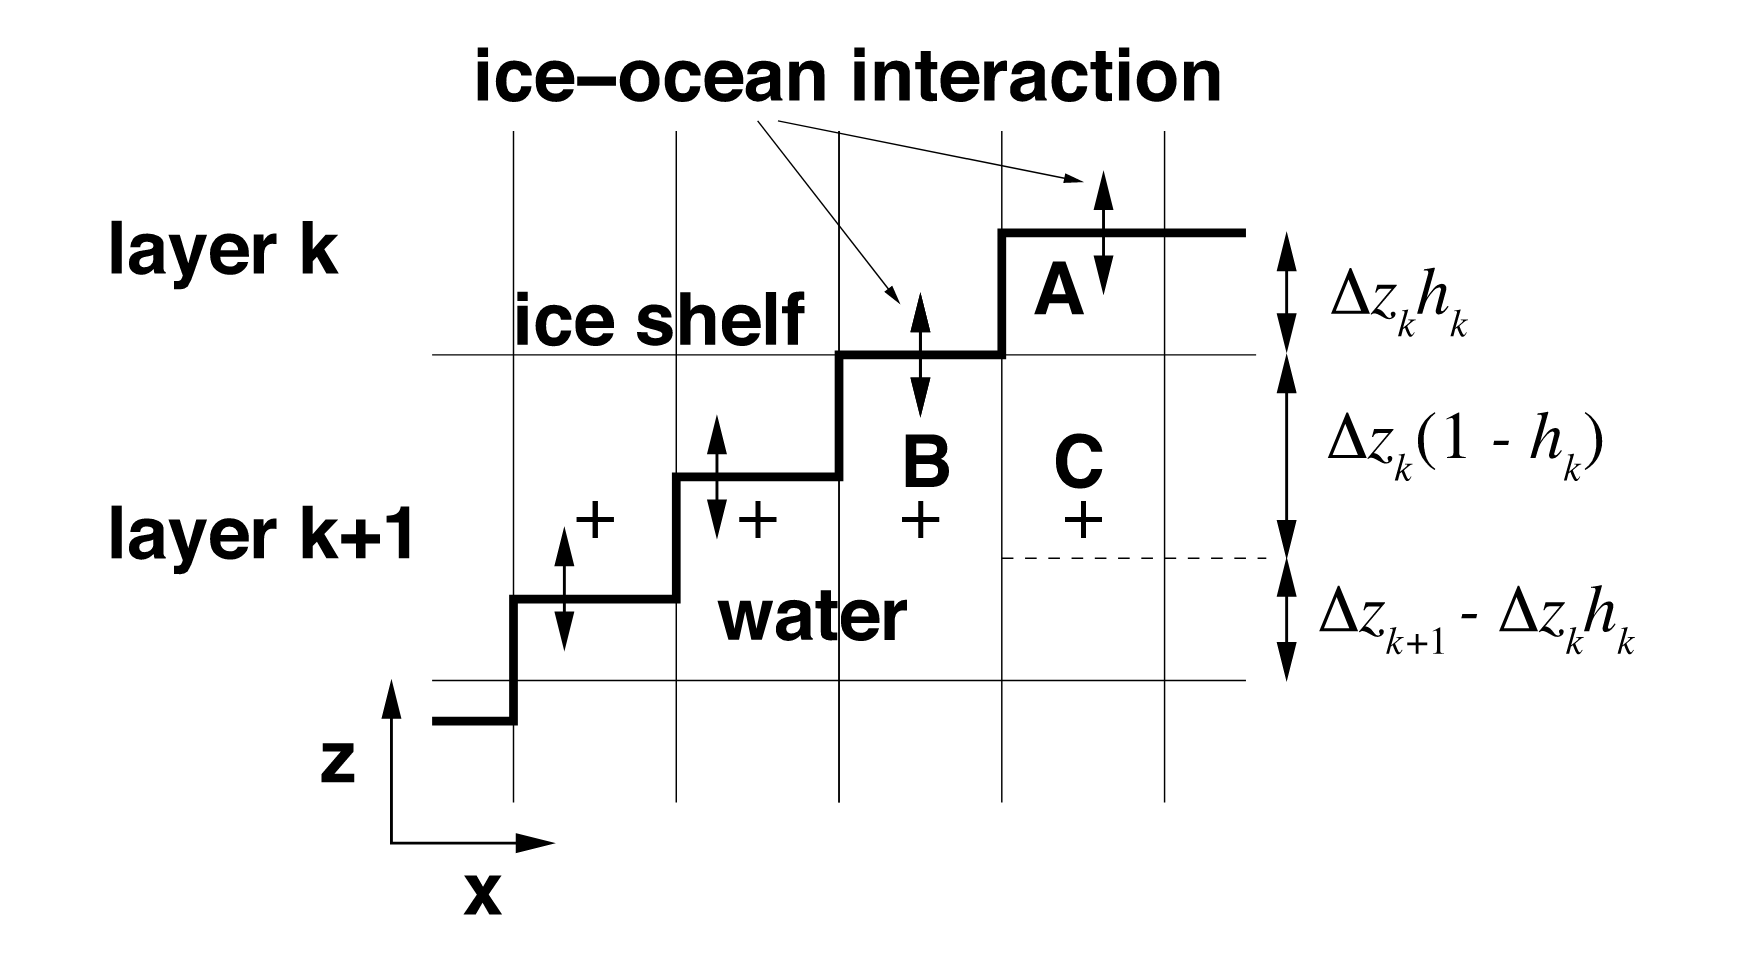
\includegraphics[width=0.7\textwidth]{chapters/4/melt_cells.png}
\caption[Melt schematic]{ Schematic showing the MITgcm package
`shelfice' treatment of partially filled cells at the ice--ocean interface, copied from \cite{losch2008modeling}. Vertical gridlines are thin. The thick line is the model ice shelf base.
Pressure gradient is computed at grid centres, marked as $+$ signs. computations. $h_k$ is the fraction of a cell which is filled, $h_k \Delta z_k$ is the actual cell thickness.}
\label{fig:melt_cells}
\end{figure}
%https://mitgcm.readthedocs.io/en/latest/phys_pkgs/shelfice.html

Our configuration of MITgcm used a vertical eddy diffusivity of  $5 \times 10^{-6}$ $\mathrm{m}^2$s and a vertical eddy viscosity of $1 \times 10^{-4}$ $\mathrm{m}^2$/s unless otherwise stated. We used a non-linear 7th order advection scheme with a monotonicity preserving limiter.
The Coriolis parameter $f0 = -1.446 \times 10^{-4}$ $\mathrm{s}^{-1}$ was set to be constant over the domain. This corresponds to the location of the channel, at a latitude of 82.47 S (Chapter  \ref{ch:data}). 
In the next section we outline the parameters and boundary conditions used in MITgcm model runs.

% When simulating tides, the same procedure was followed, matching the eastern BC to the upstreamexcept $U^E_T = A_t \sin(2\pi  TC /T_p)+ U^{ETA}$ and $|U^{ETA} - A_t| << 1  $
% where $T_p$, the tidal period is 12 hours. This simulates an estuary--like tidal signal similar to \cite{carroll2017subglacial}. On the ebb tide, a  there is a strong flux out of the domain at the top of the channel and a weaker flux into the domain over the middle and bottom. On the flooding tide, the top of the channel flows weakly inwards, and the bottom and middle flows weakly outwards.

\subsection{Adaptive domain} \label{sec:ablation_iterator}

In a separate experiment, we modelled a simple ice--bounded cavity allowing for the evolution of the cavity in time, simulating basal ablation. The domain shape was different from that described above in Section \ref{sec:domain}. The initial cross sectional domain shape was a downwards opening parabola 1.4 km wide with a 56 m deep water column, with an ocean floor at -680 m depth. On the downstream cross section the left half of a downwards opening parabola creates an initial slope from 0 to 56 m above the ocean floor over 2.2 km, followed by a horizontally flat section to $x=$  10 km. The domain is represented on Cartesian grid with (x, y, z) resolution of (50, 25, 170 m) so cells are (204, 67, 4 m) respectively.

The model was spun up for 7 days with no prescribed flux, temperature, or salinity at the boundaries, followed by a 5 day spin up with boundary condition described in Table \ref{tab:model_runs}. The model was then iterated over 500 times. At each iteration, the ocean model was run for 10 days with initial conditions as the final timestep of the previous iteration. Next, melt rate was multiplied by 10 days to calculate a basal mass balance over the period. This balance was added to the ice bathymetry and a new domain shape was created. Boundary conditions for the next iteration were recalculated so that they represented the new domain shape.

\section{Results}

% \subsection{Figs:}

% - compare model runs - sum melt rate in time
% - Medium velocity - circulation, %don
% - weak inflow show layers in TSU over time % don
% - medium velocity inflow melt from 17C showing accretion % don
% - surge flow Melt rates: do melt from  17X before and after surge. % don
% - fresh output, compare melt rates and salinity accross fresh output and medium velocity inflow and high velocity inflow
% - adaptive domain, show 3d growth of domain, 4 panel.  % don

% - Domain
% - BCs
% - control - circulation, 
% - weak inflow show layers in TSU over time
% - Fresh inflow show layers in TSU over time
% - medium velocity inflow melt from 17C showing accretion
% - surge flow Melt rates: do melt from  17X before and after surge. 
% - fresh output, compare melt rates and salinity accross fresh output and medium velocity inflow and high velocity inflow
% - adaptive domain, show 3d growth of domain, 4 panel.


\subsection{Control} \label{sec:control_run}
% #17

After 100 days of simulation, the `Control' run, with zero flow through boundaries at the entrance and exit of the channel, has developed a steady circulation pattern.
Water flows down the true right side of the cavity and up the cavity on the true left, with highest velocities ($\approx 1$ cm/s) at wide sections of the channel W1, W2 and W3, where circulation cells have formed. Two circulation cells form in each wide section of the cavity, separated at the local maximum in width. At W1, W3 and the upstream cell of W2, these cells move anticlockwise. In contrast, at W2 the downstream cell is moving weakly against background flow in the clockwise direction.   At this point in time, temperature and salinity profiles are linear with depth. Temperature ranges from -2.15 $^{\circ}$C at the top of the cavity to -2.0 $^{\circ}$C at the bottom. Salinity increases from 34.68 g/kg to 34.72 g/kg from the top to bottom. 
Basal ablation is generally low, median ablation is 0.04 m / a. Ablation is greatest ($\approx$0.5 m / a) in the deepest sections of ice at the flanks of W1, W2 and W3, where ice is in contact with warmer saltier water.

\subsection{Weak inflow of fresh water} \label{sec:weak_BC_results}
% #17A

\begin{figure}[!ht]
\centering
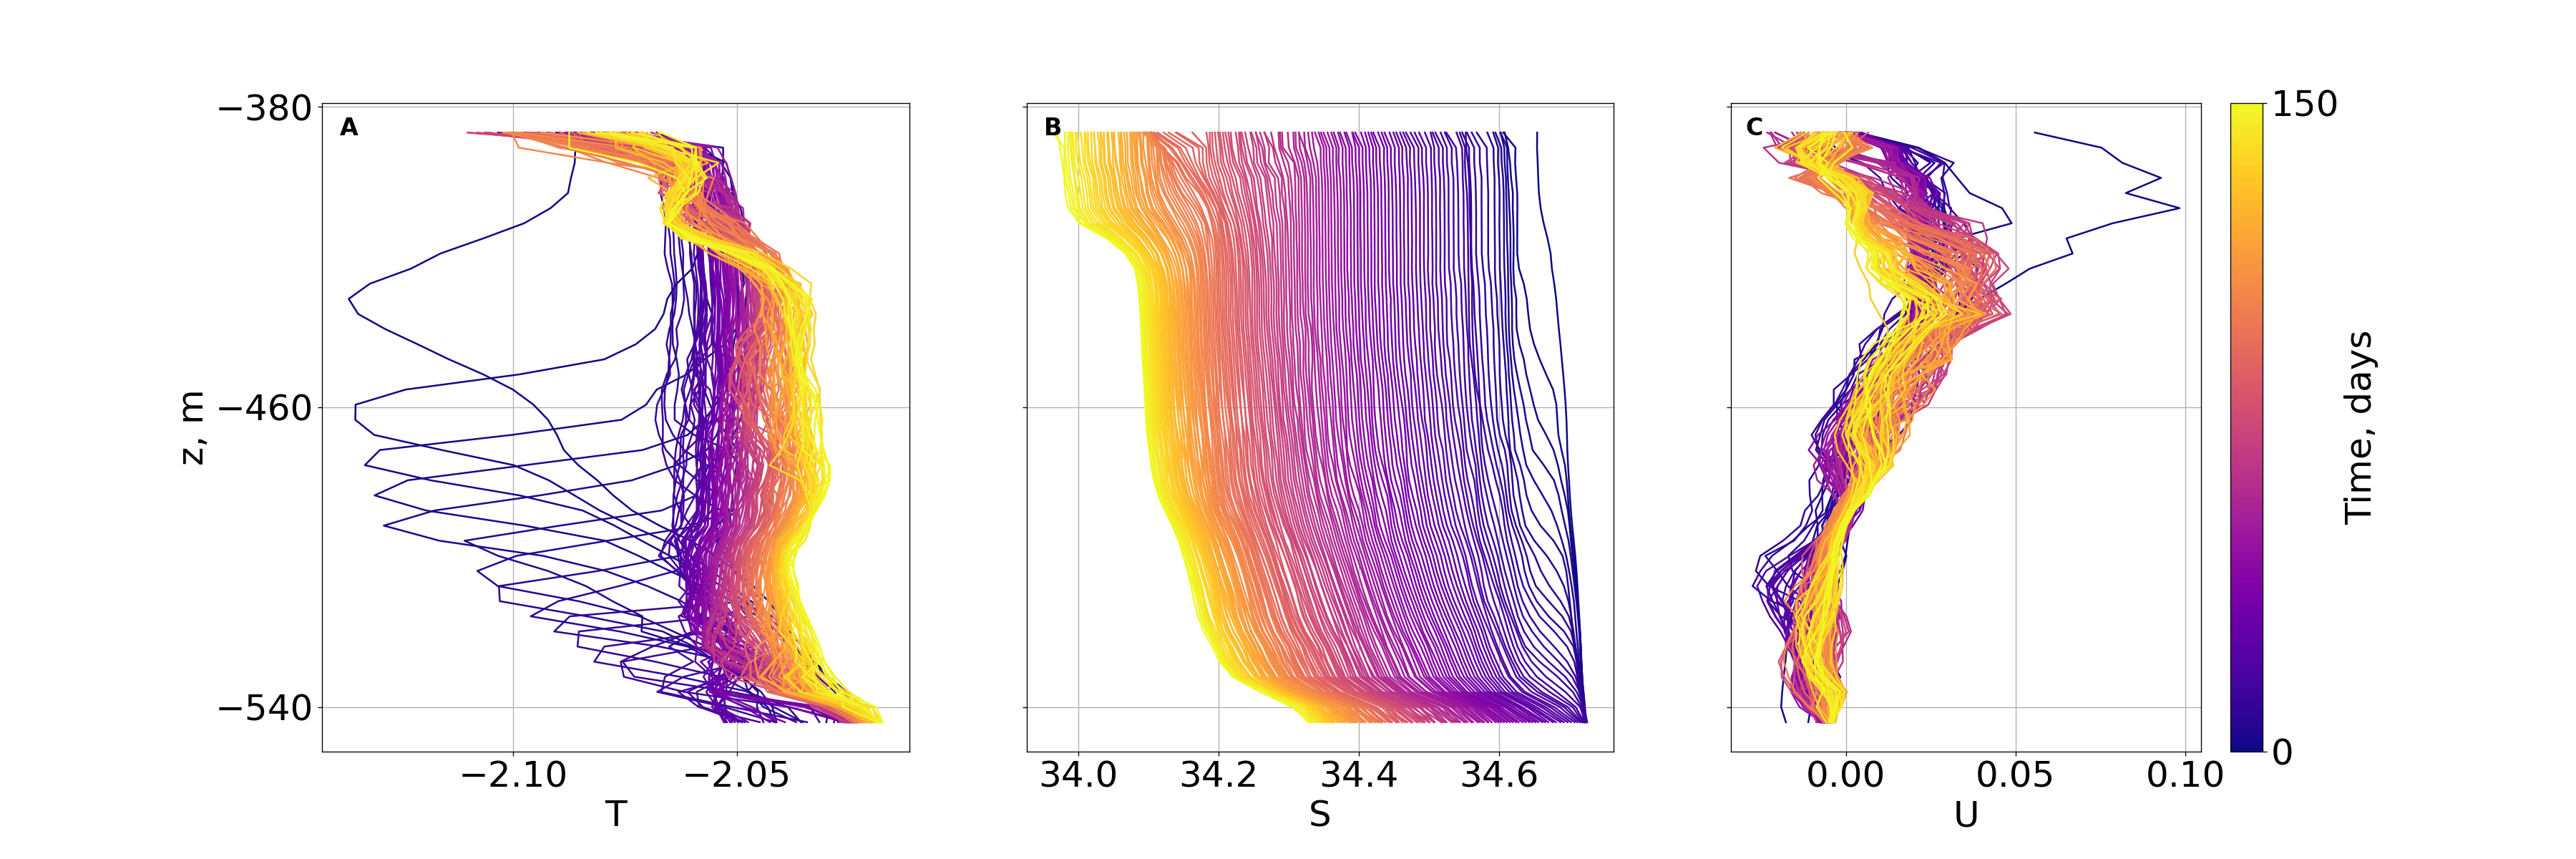
\includegraphics[width=1\textwidth]{chapters/4/weak_inflow_TSU.png}
\caption[Weak inflow (T,S,U)]{Vertical profiles of temperature (T), salinity (S) and x--component of velocity (U) over 150 days of the model run `Weak inflow'. Location of the profile is shown by the black `X' in Figure \ref{fig:domain}}
\label{fig:weak_inflow_TSU}
\end{figure}

The model run `Weak inflow' (detailed in Section \ref{sec:model_runs}) features an upstream boundary condition with relatively fresh water flowing into the cavity at 0.4 mm/s. The cavity's initial salinity and temperature are from the spun up `Control' run.
The weak inflow of relatively fresh water from the upstream boundary introduces a fresh layer to the cavity. The layer flows downstream at 5 cm/s at the top of the water column and has temperature and salinity of -2.05 $^{\circ}$C and 34.62 g/kg respectively. Underneath this layer, water is unchanged from initial conditions taken from `Control' (Section \ref{sec:control_run}). After one day, the fresh layer spans from the roof of the cavity to a depth of -475 m, at D1 and -425 m at D2 and but does not reach as far downstream as D3. It takes six days for the layer to extend downstream to the downstream boundary. By day six the layer has a horizontally uniform bottom boundary at -500 m. The layer boundary is shown in Figure \ref{fig:weak_inflow_TSU} A as the sharp corners to the true left of the plot. Over time this corner descends the water column, showing the thickening of this layer.  This bottom boundary continues to lower until at around 20 days the inflow has flooded the cavity and stabilised, and no remnant of the initial conditions are visible.  
The inflow of fresh water corresponds to a region of strong basal ablation, initially up to 7 m/yr at the upstream boundary of the channel and 1 m/yr over larger regions in the channel centre at D2 and D3. By day six ablation has reduced to 0.75 m/yr at the upstream boundary. After around 20 days, ablation decreases in magnitude in the centre of the channel and remains in the deeper ice at the flanks of the cavity. For the next 150 days ablation slowly decreases, with an upper decile 0.6 m / a as the cavity water freshens with an inflow of fresher water (Figure \ref{fig:compare_melt_sum}). 

By 20 days the salinity profile is smooth from 34.5  g/kg at the top of the water column to 34.7 g/kg at the bottom across the water column. There are no distinct layers with the exception of pockets of freshwater which accumulate at the ice boundary first at D3 then after more time at D2. After 150 days these pockets of fresh water are 40 and 15 m thick, and 34.0 g/kg and 34.1 g/kg at D2 and D3 respectively. After 20 days the cavity's temperature is relatively homogeneous, but starts to develop three layers. These layers become more distinctive over time. At 150 days water adjacent to the ice is relatively cool, -2.08 $^{\circ}$C and -2.05 $^{\circ}$C at D2 and D3 respectively. Beneath this cool layer, a warm layer (-2.03 \textdegree C) associated with the downstream flowing layer mentioned below sits between -410 m and -480 m. The bottom layer's temperature increases smoothly with depth from around -2.04 $^{\circ}$C to -2.02 $^{\circ}$C at the ocean floor at -545 m.  

Circulation after 150 days is dominated by a downstream flowing layer moving at 2-5 cm/s in the top true right of the cavities cross section, and upstream flow at a similar speed in the bottom true left.  This excludes the top 30 m of water in regions D1 and D2, which have water flowing upstream at around 5 cm/s. 
% The top of D2 has a smaller circulation within it, with water flowing downstream at the ice face and downstream immediately below.
A plume has developed on the initial positive gradient of the cavity, with vertical velocities up to 5 cm/yr. The plume is initiated from the upstream boundary at -475 m and raises to -425 m where it appears to detach and form the downstream flowing layer.
With an inflow of relatively warm fresh  water the temperature and salinity over the cavity do not converge but continue to change after 150 days, reaching median values of -2.037 and 34.15 respectively.

\subsubsection{Model variations}
This model run was repeated with an increase in vertical eddy diffusivity, which increases vertical mixing. After 150 days this results in a bottom layer 0.05  g/kg fresher than the model run with smaller vertical eddy diffusivity. This is the only noticeable effect of this change other than a general smoothing of conditions in the model output. 

Additionally, the model was repeated with a downstream (downstream) boundary condition designed to simulate estuarine tidal flow. Velocities at the top of the boundary oscillated with a tidal period ranging from strong outflow to very weak inflow. Velocities at the bottom of the boundary were selected so that the downstream boundary had a net outflow of water to conserve mass with the upstream boundary flow. This boundary condition change had no noticeable affect on the model cavity.

\subsection{Fresh inflow of water} \label{sec:fresh_inflow}
% #17B

\begin{figure}[!ht]
\centering
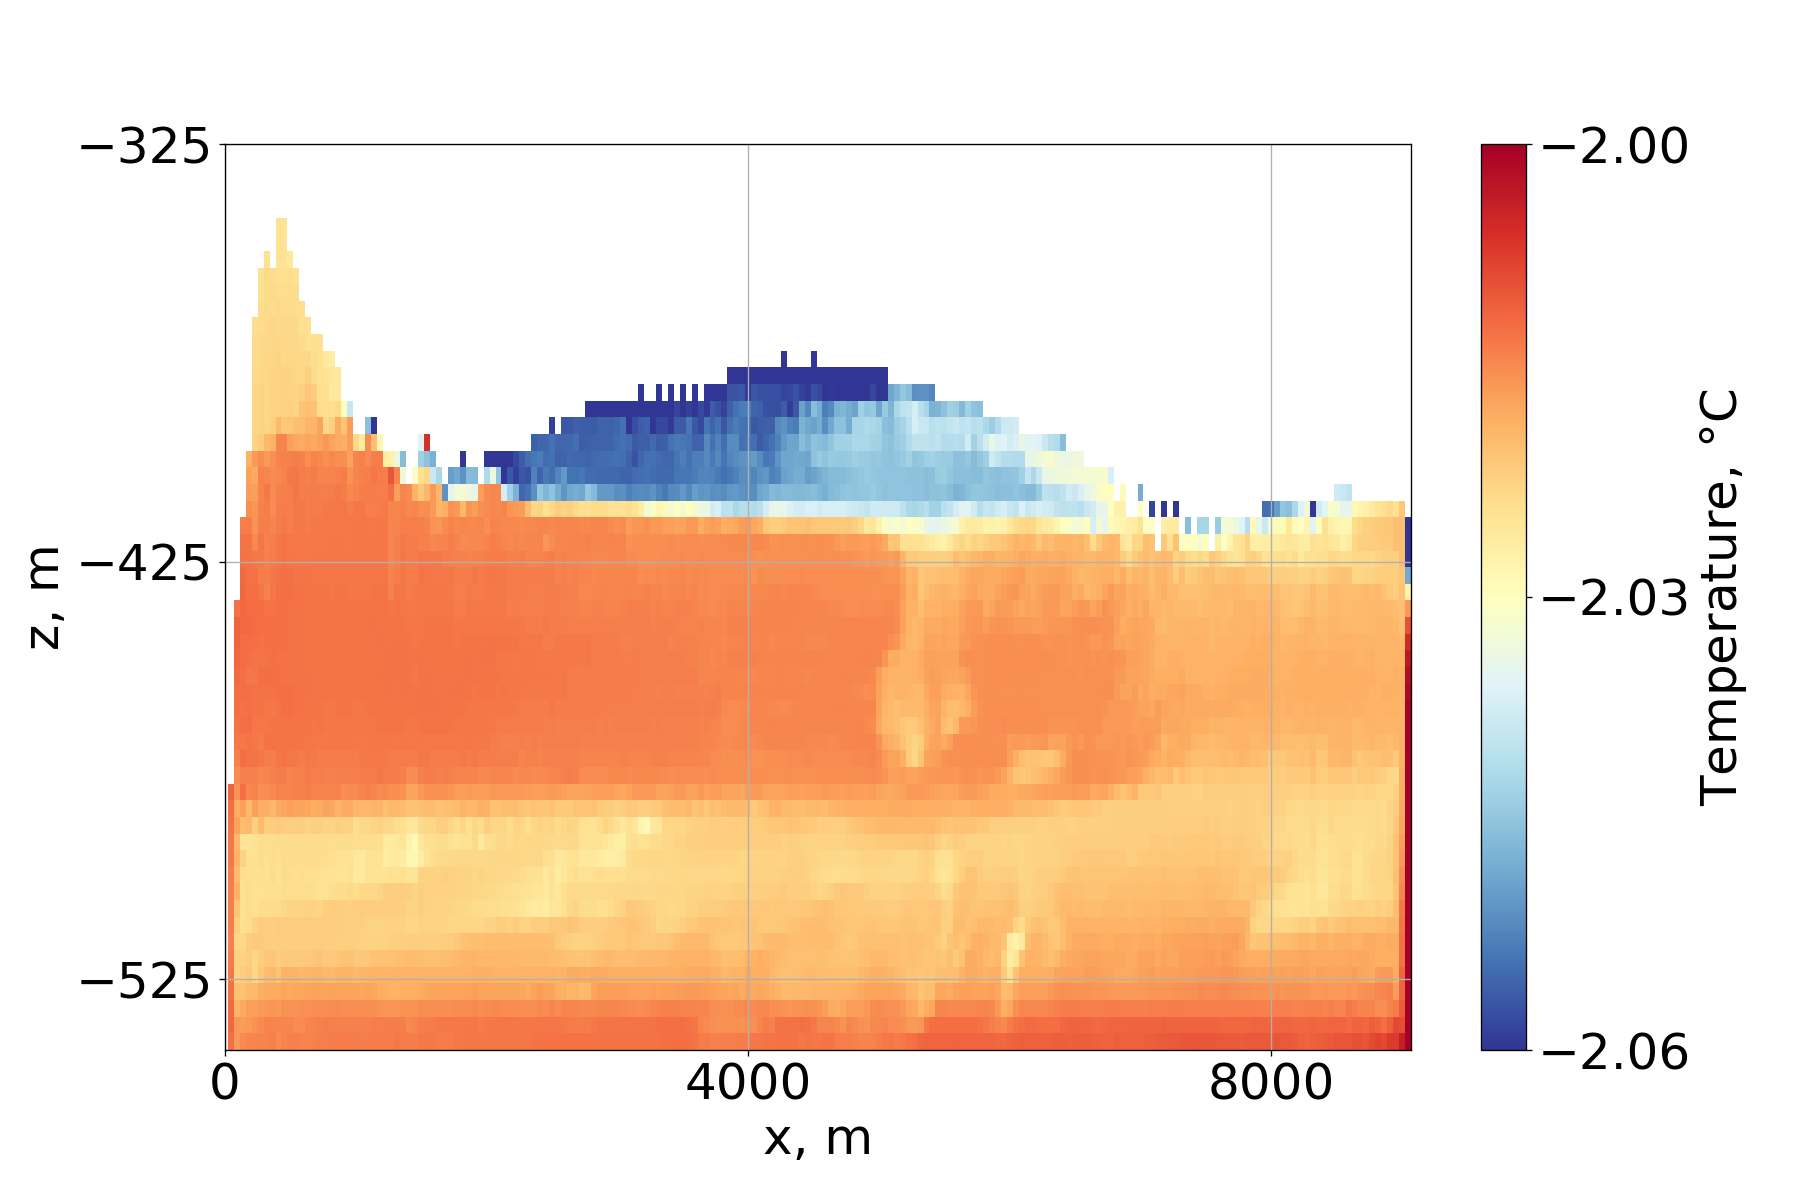
\includegraphics[width=1\textwidth]{chapters/4/fresh_input_T.png}
\caption[Fresh input (T)]{Temperature for `fresh input' at 150 days profiling the apex of the channel.}
\label{fig:fresh_input_T}
\end{figure}

The model run `Fresh inflow' is similar to the run `Weak inflow' except that the inflow of water at the upstream boundary has zero salinity (detailed in Section \ref{sec:model_runs}). Results are very similar to that described in Section \ref{sec:weak_BC_results}, except that the model ocean cavity gets more fresh in less time.
The initial fresh layer has temperature and salinity of -2.05 $^{\circ}$C and 34.5  g/kg respectively.  By day five the layer has horizontally uniform bottom boundary at -500 m, and it takes around 15 days for the layer to flood the cavity.

\begin{figure}[!ht]
\centering
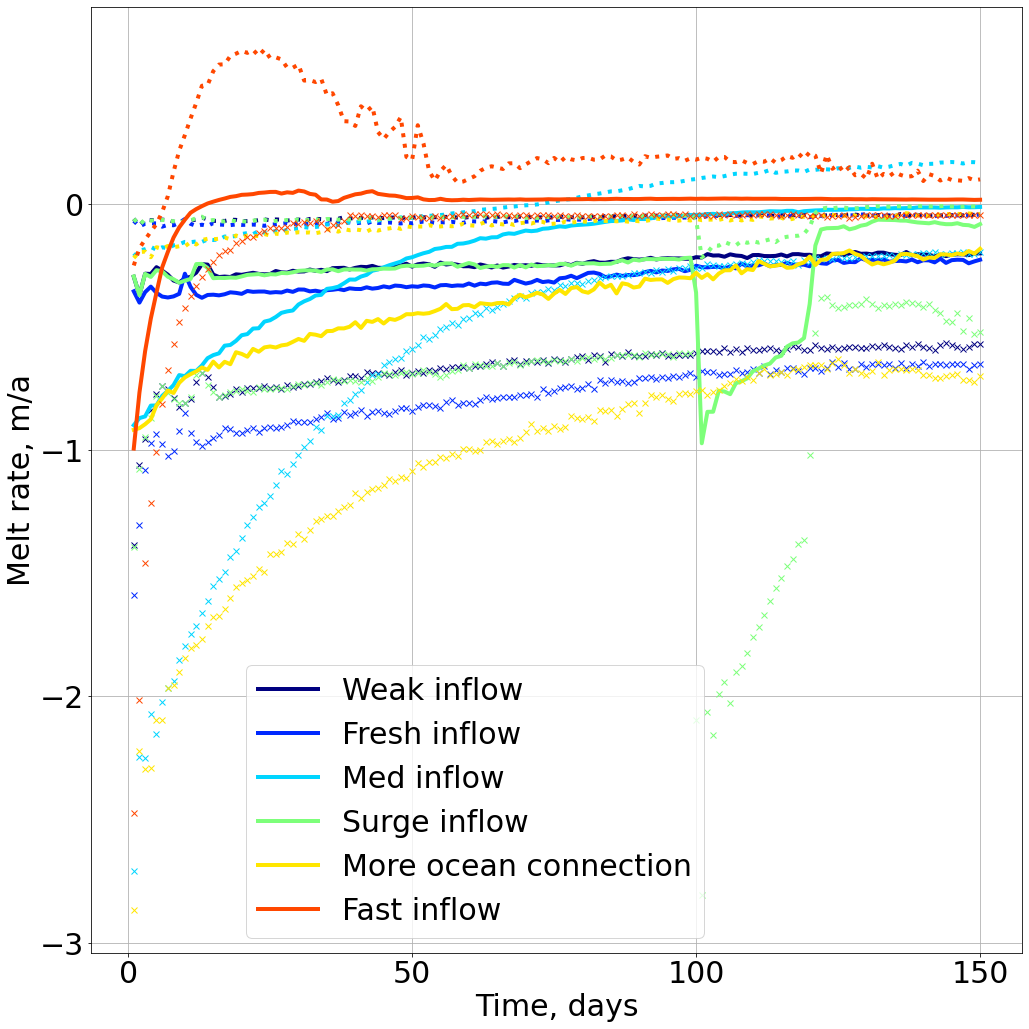
\includegraphics[width=1\textwidth]{chapters/4/compare_melt_sum.png}
\caption[Melt sum comparison]{Time series of basal mass balance over the domain for each model run. Model run colour shown in legend, dotted lines with squares and x's show the lower and upper deciles for mass balance respectively. Solid lines show median mass balance.}
\label{fig:compare_melt_sum}
\end{figure}


Basal ablation is as high as 9 m/yr at the downstream boundary of the channel, with a top decile of 1.5 m/yr which represents large regions in the channel centre around D2 and D3. By day five the top decile of ablation is reduced to 1 m/yr, and over the next 150 days  slowly decreases to 0.7 m / a as the cavity water freshens (Figure \ref{fig:compare_melt_sum}).
The salinity and temperature profiles follow the same trend as described in Section \ref{sec:weak_BC_results}, though with slightly fresher profile. By 150 days salinity ranges from 33.5 g/kg to 33.9 g/kg at depth, with a large pocket of relatively cool water developing at the channel ceiling. This layer ranges from 33.4 g/kg at D2  to 33.3 g/kg at D3 (Figure \ref{fig:fresh_input_T}. 
Circulation is indistinguishable from that described in Section \ref{sec:weak_BC_results}. 
With an inflow of relatively warm fresh  water the temperature and salinity over the cavity do not converge but continue to change after 150 days, reaching values of -2.02 \textdegree and 33.6 g/kg respectively.

% # Huge input 10 cmps has high meltrate
% # 16C has freezing in middle


\subsection{Medium velocity inflow} \label{sec:medium_inflow}
% # 17C

The model run `Medium inflow' (detailed in Section \ref{sec:model_runs}) features inflow water at the same temperature and salinity as `Weak inflow' (-1.2 $^{\circ}$C and 16.5 g/kg), but with a faster velocity, of 1 cm/s at the upstream boundary. The change in velocity of the boundary forms an initial plume with much greater melt rates, and the cavity freshens much faster, to the extent that accretion occurs in the the channel centre (Figure \ref{fig:accretion} and Figure \ref{fig:compare_melt_sum}).

\begin{figure}[!ht]
\centering
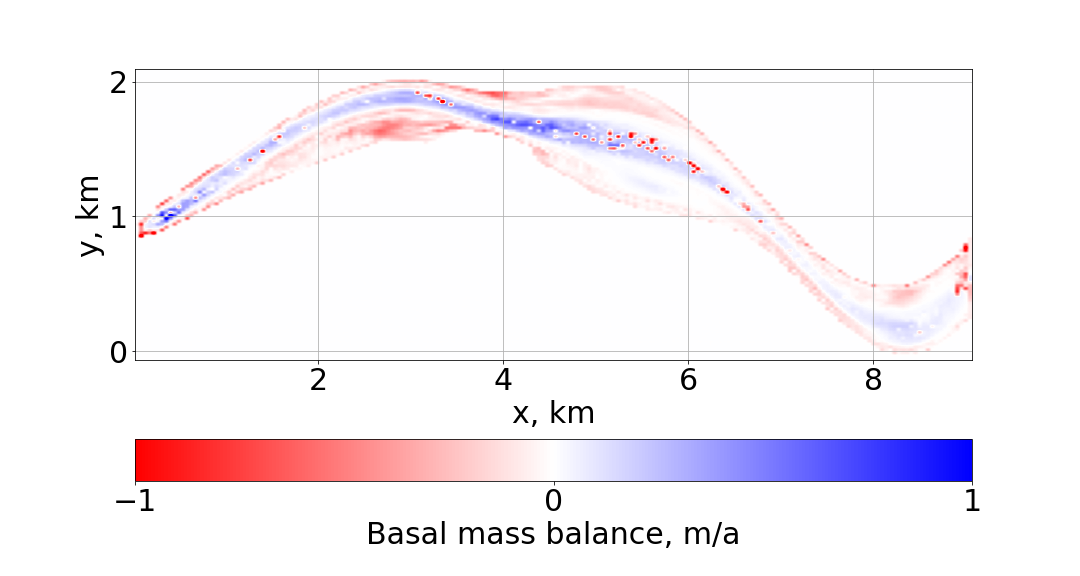
\includegraphics[width=1\textwidth]{chapters/4/accretion.png}
\caption[Medium inflow (melt)]{Ice shelf basal mass balance from `Medium inflow' at 150 days}
\label{fig:accretion}
\end{figure}

The initial inflow of water forms a fresh layer with temperature and salinity of -2.02 $^{\circ}$C and 33.6  g/kg, which takes 2-3 days to reach the downstream boundary of the model. By day 7, this inflow has flooded the cavity.  
For this initial period, a plume causes ice ablation of up to 20 m/yr over a small area at the downstream boundary. The top decile of ice ablation is 3 m/yr of melt which is focused around the centre of the channel and extends down the length of the channel. As the cavity freshens, ablation decreases until it plateaus after around 80 days, with a top decile of 0.3 m/yr (Figure \ref{fig:compare_melt_sum}). This coincides with water freshening to the pressure melting point at the top of the channel. At this time, basal accretion starts to occur, and by 150 days accretion of up to 1.4 m/yr occurs at inception of the channel. Accretion is focused at the top of the water column at the centre of the channel 90-200 wide down the whole length. This region is represented by the top decile of basal accretion which is 0.3 m/yr. Ablation continues to occur on the deeper parts of the ice on either side of the channel, as large as 2 m / a. Despite accretion occuring, net basal mass balance is positive after 150 days.

Circulation for `Medium inflow' is shown in Figure \ref{fig:medium_flow_circulation}, and is typical of most model runs.
In the upstream half of the cavity, water flows downstream in the top half of the cavity (-350 m to -475 m depth) at around 3-5 cm/s and flows back upstream at the bottom half. In the downstream half of the cavity, at the wide parts of the cavity W2 and W3, weak horizontal convection cells form. The downstream flow trends to the top true left side of the cavity and water flows upstream at the top true right. In the narrow section of channel between W2 and W3 the top half of the water column flows uniformly downstream. 
The bottom layer of the cavity mostly flows upstream, though also features weak horizontal convection cells at W2 and W3 with a clockwise flow at -510 m and an anticlockwise flow at -535 m deep. 

\begin{figure}[!ht]
\centering
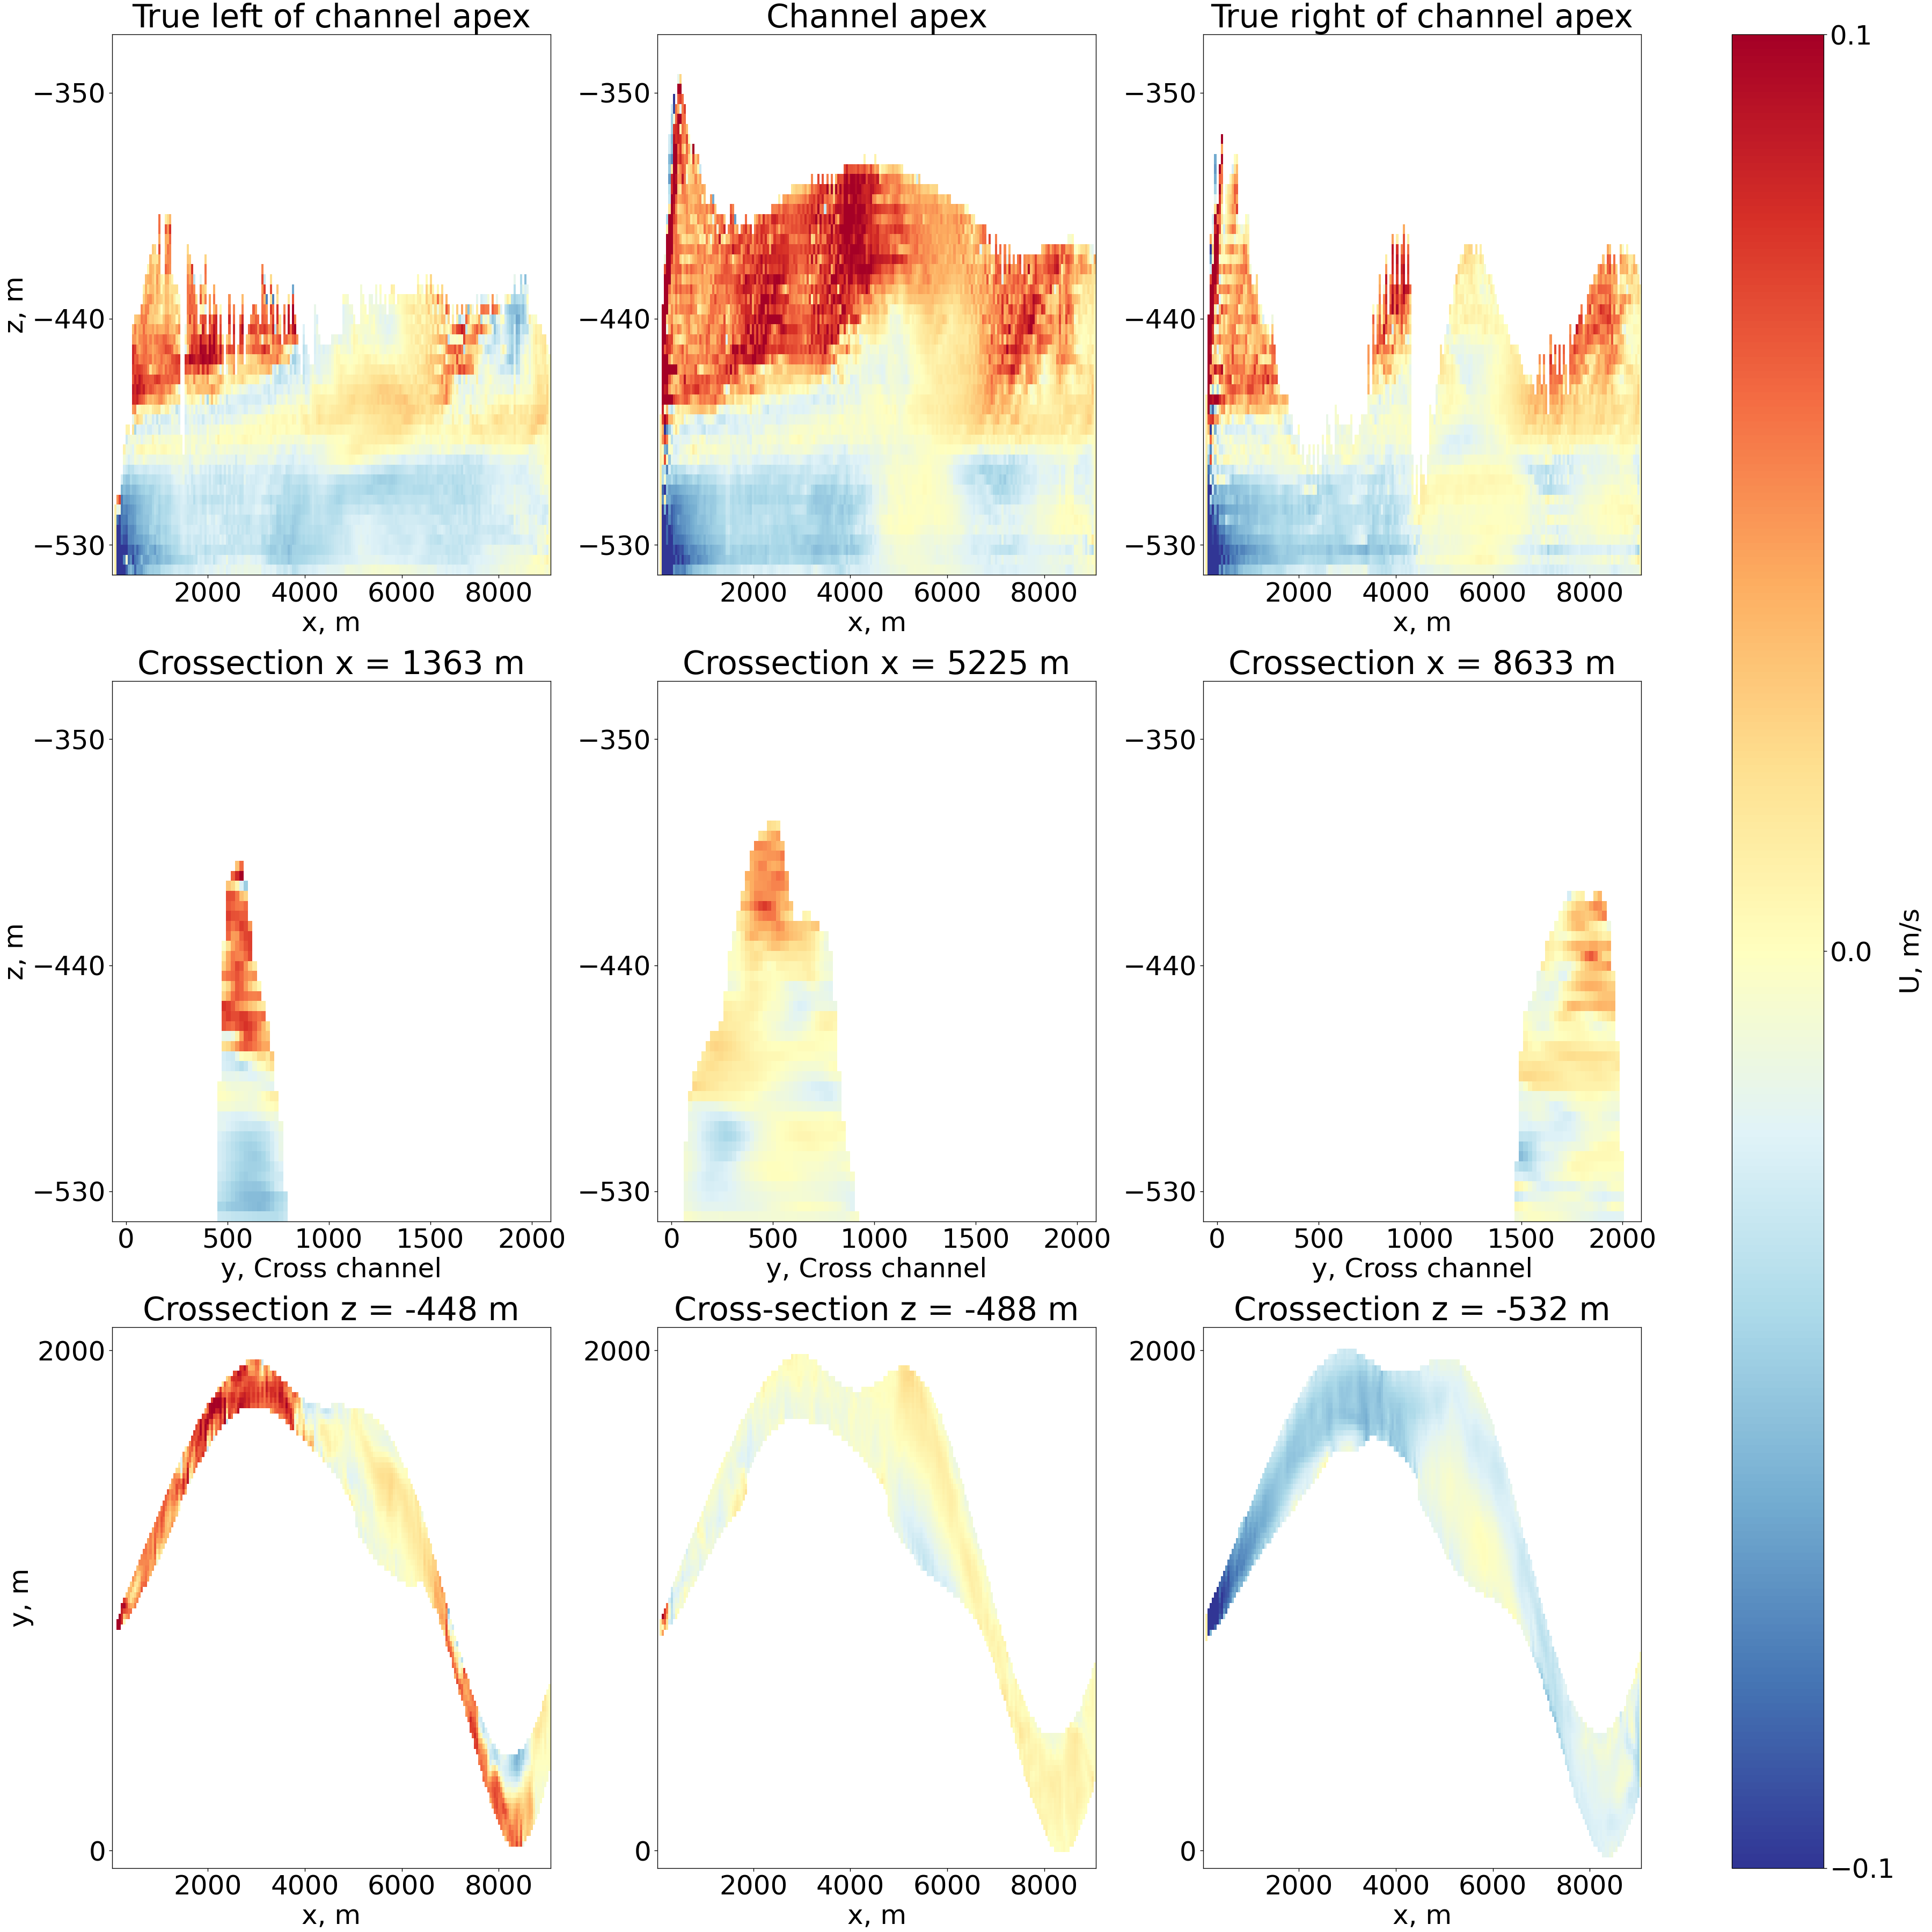
\includegraphics[width=1\textwidth]{chapters/4/medium_flow_circulation.png}
\caption[Medium inflow (U)]{U (x--component of velocity) from `Medium inflow' at 150 days. Note that axes are not equal scale.}
\label{fig:medium_flow_circulation}
\end{figure}


Temperature and salinity through the cavity do not converge but continue to change after 150 days. Temperature and salinity do not show any layers, varying from -1.43 $^{\circ}$C and 21  g/kg at the top to -1.5 $^{\circ}$C 21.8  g/kg at the bottom. 

\subsection{Surge inflow} \label{sec:surge_inflow}



%17X
% 100 days at 17A followed by 20 at C
The model run `Surge inflow' runs for 100 days with boundary conditions the same as `Weak inflow' followed by a 20 day surge period with boundary conditions from `Medium inflow'. At 100 days, the model looks like `Weak inflow', and the top decile of ablation is 0.6 m/yr (Figure \ref{fig:compare_melt_sum}). Water is around -2.04 $^{\circ}$C, except for a cool layer at the top and a layer 0.02 \textdegree C warmer in the bottom 10-20 m. Salinity is stable with depth, a fresh layer 10-20 m deep sits on top of a layer smoothly increasing from 34.2 g/kg to 34.4 g/kg at the sea floor. Water moves downstream in the top half of the water column at up to 4 cm / a and upstream in the bottom half at up to 2 cm / a. 

The surge of fresher, warmer water takes two days to fill the length of the channel, at which point basal ablation reaches up to 17 m/yr over a small area at the head of the channel and a top decile of 2.8 m/yr (Figure \ref{fig:compare_melt_sum}) representing ablation down the centre of the channel (Figure \ref{fig:surge_melt}). Velocities as high as 20 cm/yr and 8 cm/yr flow downstream in the top half and upstream in the bottom half of the cavity respectively. After 5 days these velocities weaken by around 25\%. After 2 days of the surge, the top half of the water column is filled with water around -2.01 \textdegree C and 33.5 g/kg. This layer is fresher and warmer closer to the upstream boundary the channel. Cooler saltier water remains beneath the layer. After 5 days of surge  the distinctive bottom layer is not visible. For the remainder of the surge, the ocean conditions become more homogenous. After 20 days of surge, the water column smoothly increases in salinity from  32.0 g/kg at the sea floor and converges to 30.5 g/kg at the top of the water column. Temperature warms from -1.9  \textdegree C at depth to -1.95 \textdegree C.

\begin{figure}[!ht]
\centering
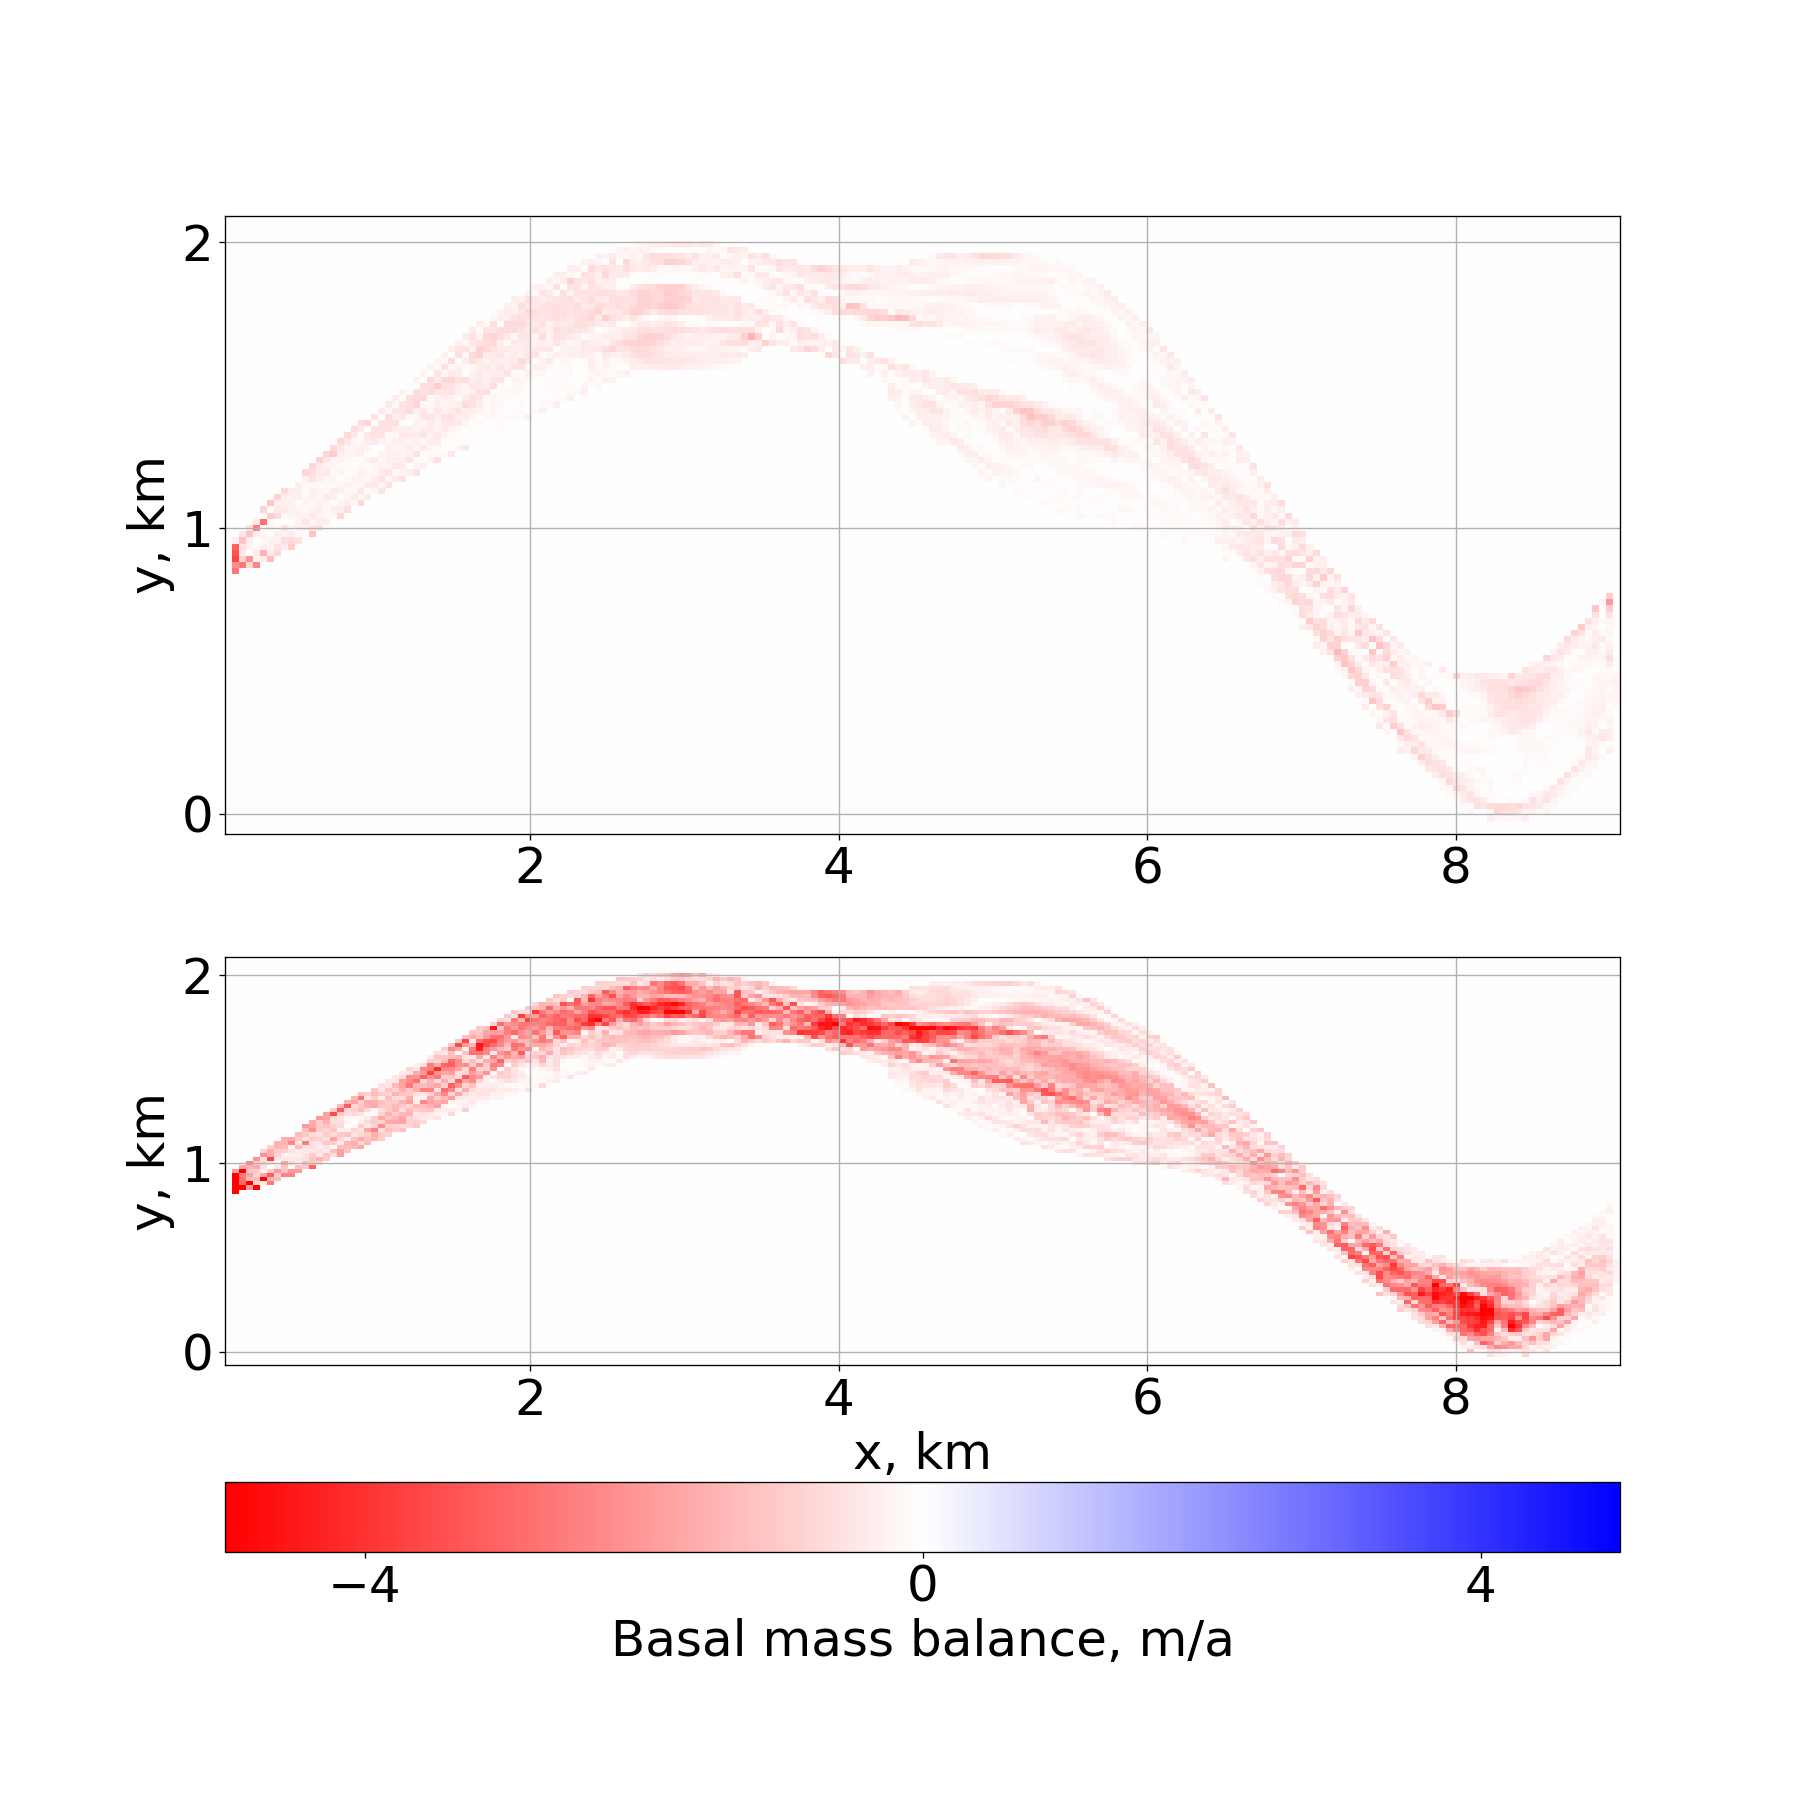
\includegraphics[width=1\textwidth]{chapters/4/surge_melt.png}
\caption[Surge inflow (melt)]{Basal mass balance of the model ice shelf showing `Surge inflow'. Top: Basal mass balance at 99 days before the surge in inflow velocity. Bottom: Basal mass balance at 101 days during the surge in inflow velocity. See Figure \ref{fig:compare_melt_sum} for time series of median melt over the surge.}
\label{fig:surge_melt}
\end{figure}

When the surge stops, velocities shrink to near zero at the top of the water column, triggering a drop in melt rates. The top decile of melt rates drops from around -1.4 to 0.4 m/yr (Figure \ref{fig:compare_melt_sum}). A weak flow around 3 cm/yr circulates water in a layer that spans from -450 to -540 m deep. Over the next 30 days post surge, the gradient in salinity and temperature of the bottom water shrinks as the salty bottom half of the water column becomes more homogeneous. The gradient in salinity and temperature of the top section of the water column increases as water near the top of the water column becomes fresher. Maximum and minimum temperatures and salinity at the top and bottom of the water column remain roughly the same as described above. A distinct layer forms at the top 30-40 m of the water column with temperature increasing with depth and a constant salinity of 30.5 g/kg. 


\subsection{More ocean connection} \label{sec:fresh_output}
% # 17D


\begin{figure}[!ht]
\centering
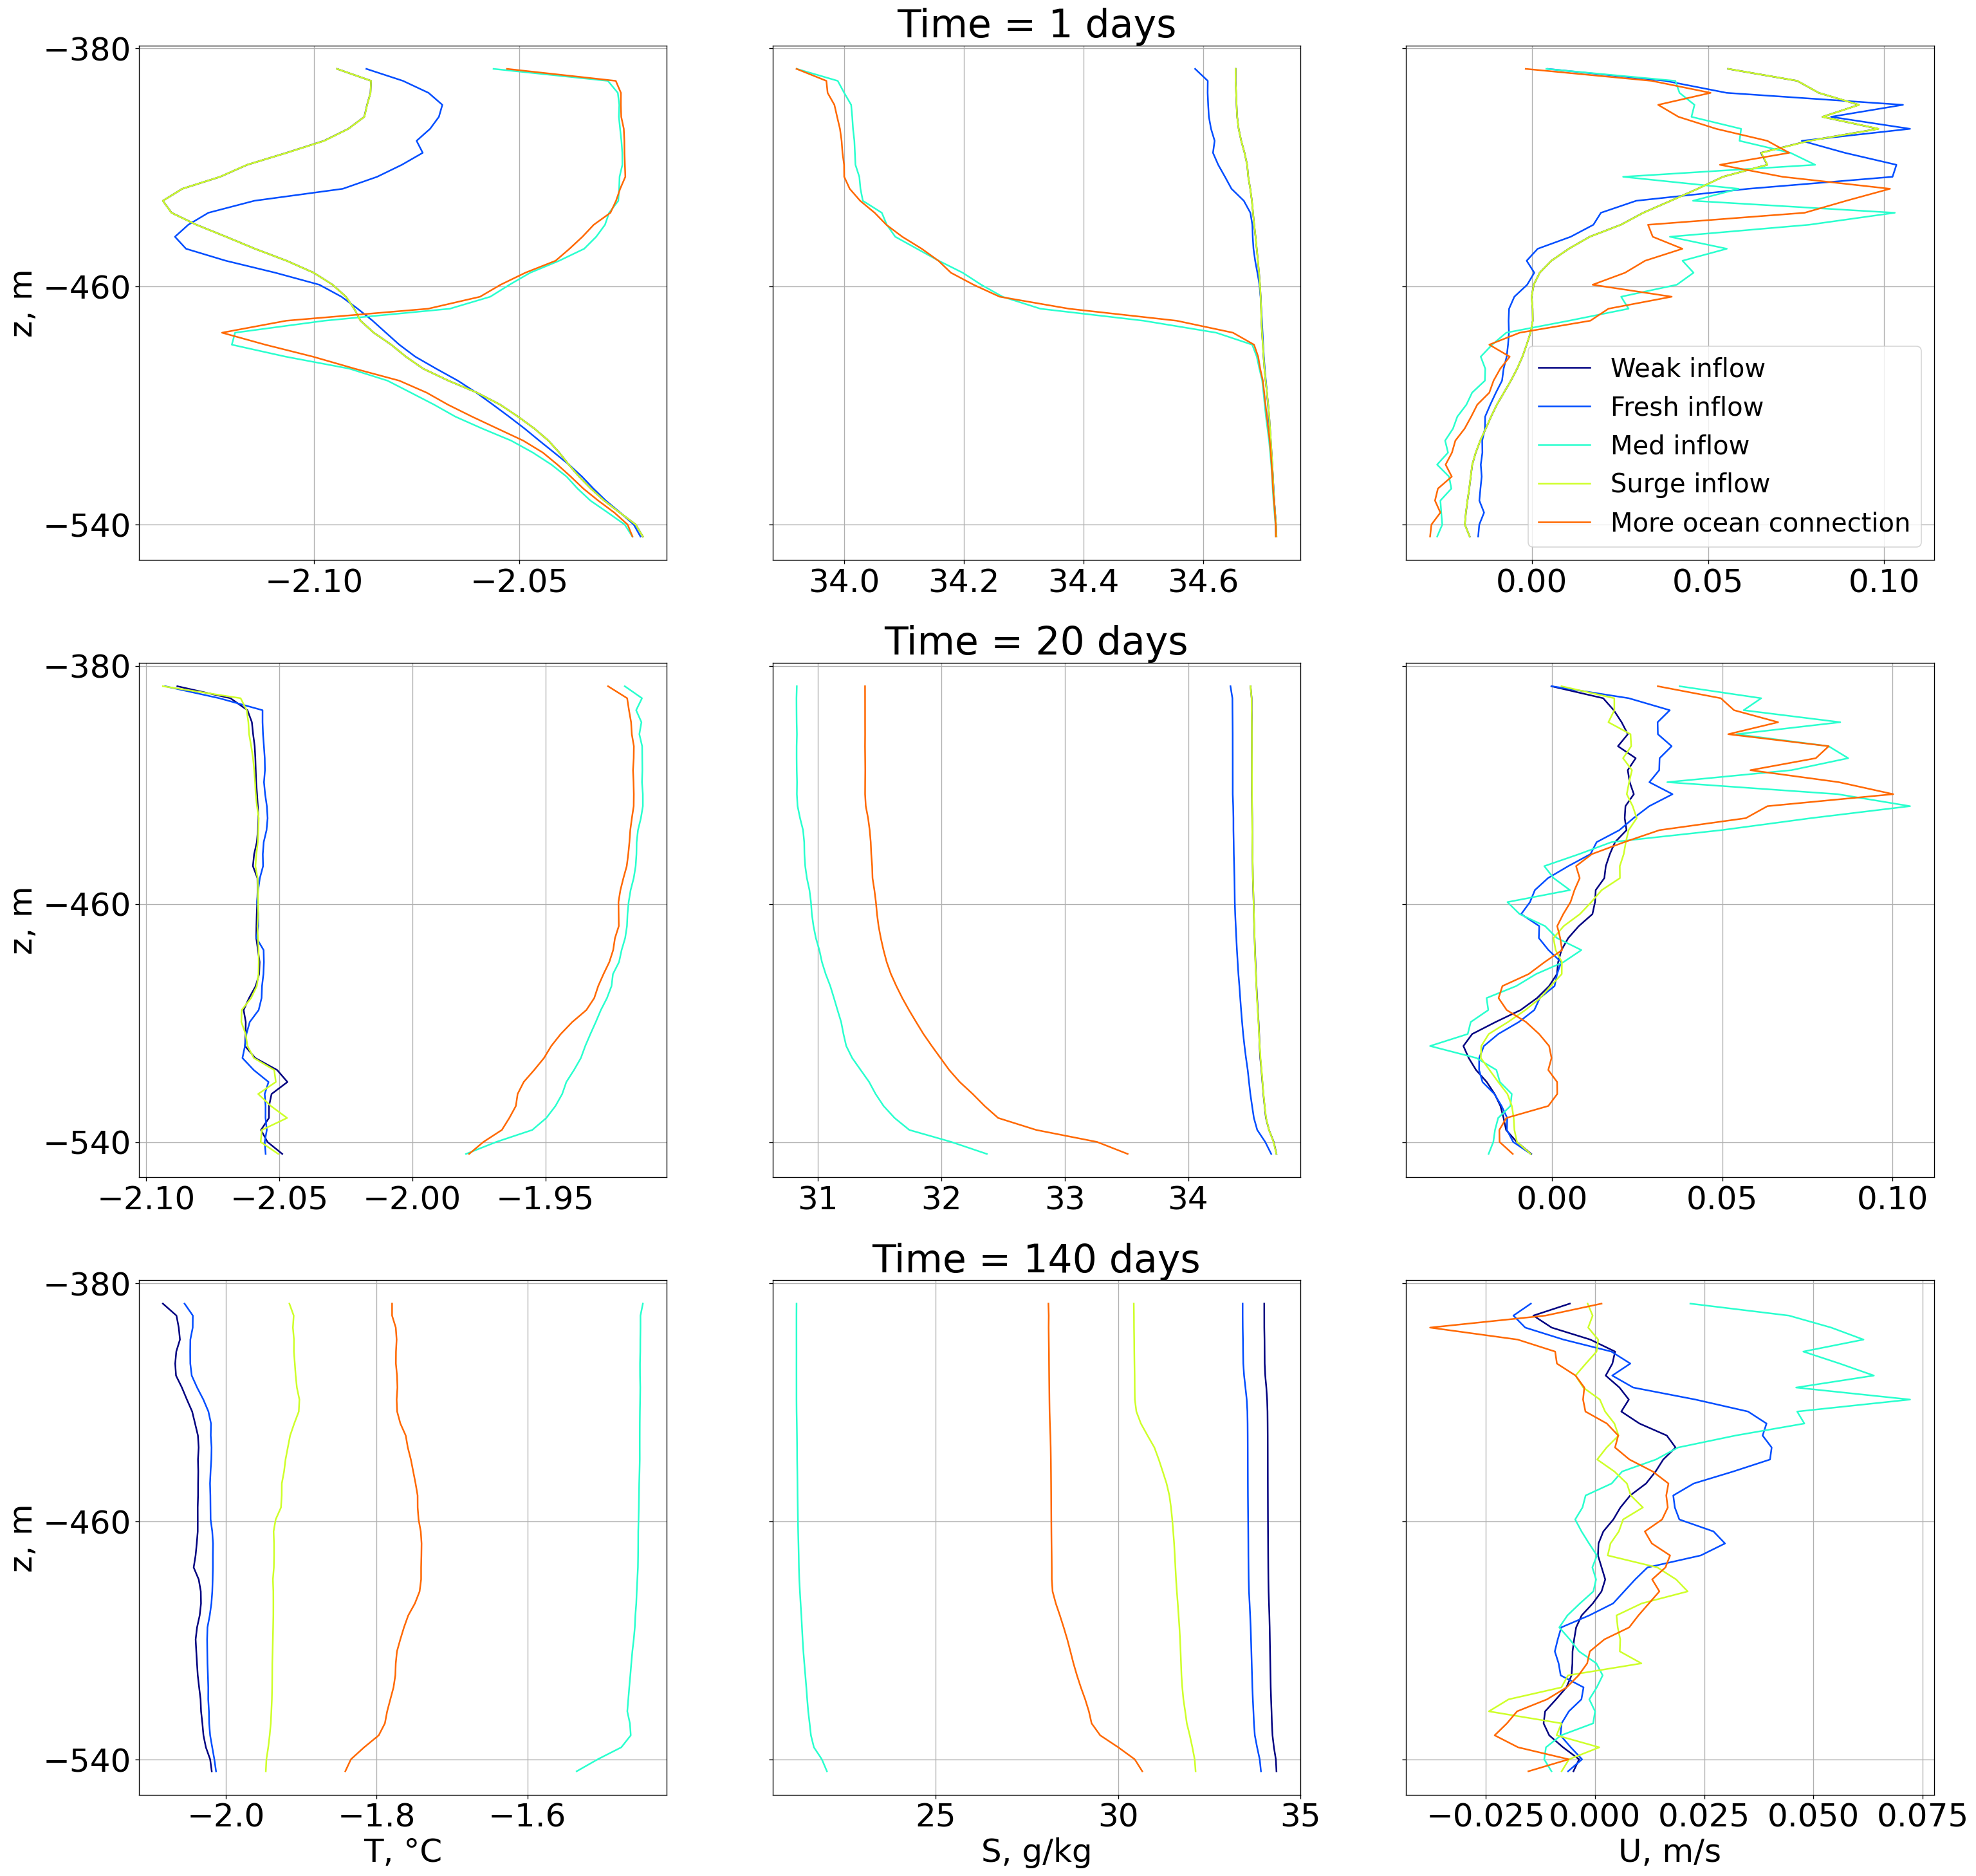
\includegraphics[width=1\textwidth]{chapters/4/compare_all_TSU.png}
\caption[All model runs comparison (T,S,U)]{Vertical profiles of temperature, salinity and x--component of velocity for all model runs at 3 points in time.}
\label{fig:compare_all_TSU}
\end{figure}

The model run `More ocean connection' has the same conditions  as `Medium inflow' (described in Section \ref{sec:medium_inflow})  except the downstream boundary condition has more circulation with the simulated larger Ross Ice Shelf cavity. Flux is stronger both outwards at the top of the boundary where water is fresher, and inwards at the bottom of the boundary where water is saltier. This has the effect of slowing the decrease in salinity in the cavity, which is caused by the inflow of fresher water from the upstream boundary. Because the inflow of fresh water in `More ocean connection' is identical to that in `Medium inflow', the first part of the model runs are indistinguishable. The longer term ($\>$ 100 days) trajectory of runs are different.

Unlike the run `Medium inflow', temperature and salinity converge. At 150 days, the converged temperature and salinity varying from -1.8 $^{\circ}$C and 28  g/kg at the top to -1.85 $^{\circ}$C 30.5  g/kg at the bottom \ref{fig:compare_all_TSU}. At this time, downstream flow is concentrated in a layer between -435 and -480 m. This layer is around 0.05 $^{\circ}$C warmer than water above and below. This differs from `Medium inflow', where has downstream flow is at the top of the cavity for the duration of the model run (Figure \ref{fig:compare_all_TSU}). 

The top decile of ablation, representing large areas first in the centre channel and later moving to the sides of the cavity, eventually converges to 0.75 m/yr (Figure \ref{fig:compare_melt_sum}). No accretion occurs in the model run.
Circulation differs from `Medium inflow' in that by 150 days the convection cells which develop early in the model run largely break down. The cavity develops downstream flow at the top half and upstream flow at the bottom half.

\subsection{Fast inflow} \label{sec:high_velocity}
%17F

The model run `Fast inflow' features a 10 cm/s inflow of relatively fresh water from the upstream boundary (detailed in \ref{sec:model_runs}). This run differs from other runs, in that initial conditions are taken from `More ocean connection', not from the `Control' run. The cavity starts with relatively fresh warm water, with a median of 30  g/kg and -1.85 T.  Despite this, initial melt is high, with maximum basal ablation of 15 m / a and a top decile of 2.5 m/yr (Figure \ref{fig:compare_melt_sum}). Temperature and salinity profiles initially vary from -1.75 $^{\circ}$C and 27  g/kg to -1.9 and 32.0  g/kg from top to bottom. The top half of the cavity is cooler and fresher close to the upstream boundary and the bottom half is homogeneous. These differences become after little time. From around 30 days, temperature is relatively constant with depth, at -1.3 $^{\circ}$C and 25.7  g/kg respectively. Between 40 and 45 days, the top 60 m develops distinct pockets of fresher cooler water which sit ontop of a homogeneous layer. While the top layer continues to cool and freshen for the next 100 days, the bottom layer is relatively constant at around -1.2 $^{\circ}$C and 16.5 g/kg. As in other models, the cavity shows a  downstream flow at approximately 5 cm/s in the top half of the water column and upstream flow in the bottom half. However, distinct from other models, at 40 to 45 days this layer collapses and flows under the top layer left of the channel at around 3-5 cm/s, and the top of the cavity cross section shows weak upstream flow.  

% \subsection{Tidal eastern boundary}
% % # 16U
% FRIDAY

% Really identical to 16A just freshens faster.

\subsection{Adaptive domain} \label{sec:adaptive_dom_results}

% Two model domain shapes were run in the ablation iterator described in Section  \ref{sec:ablation_iterator}. 
% We describe results from the two model runs sequentially, first describing the ocean state in the cavity and next describing the effect on melt.

\begin{figure}[!ht]
\centering
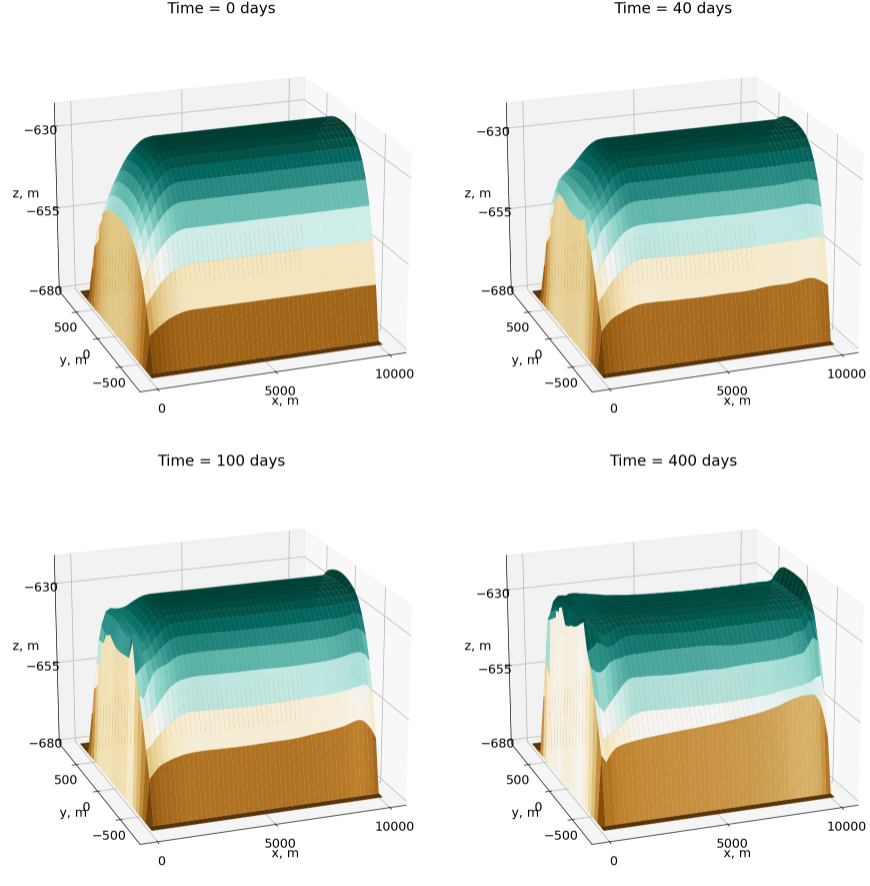
\includegraphics[width=1\textwidth]{chapters/4/adaptive_domain.png}
\caption[Adaptive domain]{The shape of a model cavity `Adaptive domain' at different points in time}
\label{fig:adaptive_domain}
\end{figure}

`Adaptive domain' has a different domain shape (Figure \ref{fig:adaptive_domain} T=0) to other model runs. Unlike all other runs, the modelled ice boundary can ablate, changing the shape of the domain through time. The upstream boundary condition has a slow influx of fresh water identical to `Fresh input'.
The spun up `Adaptive domain' features a downstream flowing layer which flows up the sloped roof at the upstream side of the cavity, flowing at up to 20 cm/s. At -640 m deep, the downstream flowing layer stops flowing up the sloped roof and detaches from the ice. It then flows horizontally down the length of the domain at around 10 cm/s, trending to the true left wall. Below this downstream flowing layer, water flows upstream. Above this downstream flowing layer, water is stagnant and relatively fresh, at 28-30 g/kg. Below this stagnant layer, salinity increases smoothly and linearly with depth from around 30.2 g/kg to 31.2 g/kg. The bottom of the downstream flowing layer does not correspond to a change in salinity. Temperature varies only slightly over the domain. While the downstream flowing layer is slightly warmer at -2.0 $^\circ$C, the background temperature is -2.02 $^\circ$C. 
The initial ice ablation pattern in the cavity shows ablation up to 4 m/yr on the upstream ramp and at the sides of the channel. Ablation is slightly stronger on the true left side than the true right.  The centre top of the cavity where the stagnant fresh water sits shows accretion of around 0.1 m/yr.

When the ice walls and roof are ablated over time, the domain changes in shape to become more square. Ablation is strongest closer to the upstream boundary, so the lower portion of the sloped roof is ablated first, losing its slope. As the leading boundary of the cavity ablates upwards, the ablation rate immediately downstream follows, because the deepest ice generally shows strongest ablation. As a result, the slope uniformly ablates upwards until it forms a flat roof. With stronger ablation on the sides of the cavity, the the cross sectional shape also becomes more square. This is partially due to limitations in the model, the model cannot ablate sides of cells, only the roofs. The cavity takes around three years to ablate to a square shape. The front roof of the cavity then continues to ablate, forming a negative gradient in the roof.

% The spun up second domain (the `pipe' detailed in Section \ref{sec:ablation_iterator}), has stronger ablation rates in the centre of the cavity. The cavity features a plume which flowsZoom to 1.02 down the centre, in the top of the water column. Salinity ranges from 29.8  g/kg at the top to 33  g/kg at the bottom of the water column. Temperature is -2.1 at the top and bottom of the water column, and is around 0.05 $^{\circ}$C cooler at mid depths. Ablation is foccussed on the walls of the 

\section{Discussion} \label{ocean_discuss}

% ! intro
% We aim to better understand and constrain ocean processes in a basal channel at the grounding zone of the Kamb Ice Stream, using an ocean model to extrapolate from the existing knowledge of the channel shape and channel melt (described in Chapter \ref{ch:data}), and nearby oceanographic observations (described in Section \ref{sec:conditions}).  
% Firstly, we aim to better constrain subglacial discharge, which we assume causes the formation of the channel (Chapter \ref{ch:data}). 
% Secondly, we aim to better describe subglacial plume dynamics by modelling melt without first making the assumption that a plume is driving melt. Lastly, we aim to understand how the channel is interacting with the open ocean, constraining the connection between the channel cavity and the open ocean. 

% How can MITgcm constrain ocean processes in cavity, given the estimations of melt and accretion from previous chapter?
% 1. constrain subglacial discharge. 
% 2. describe subglacial plume dynamics.
% 3. channel open ocean connection, constraining the connection between the channel cavity and the open ocean. 

\subsection{Constraining ocean processes}

This research aims to better constrain the cavity conditions, using the MITgcm ocean model to extrapolate from the observations described in Chapter \ref{ch:data}. In particular, we aim to better constrain subglacial discharge, meltwater plume dynamics and the connection between the channel and the ocean.

In Chapter \ref{ch:data}, we identified a 200 m x 1.5 km region of basal ablation around the inception of the channel. We estimated the region to have ablation rates over 20 m/yr. 
While the model runs showing the strongest ablation successfully reproduce rates of 20 m/yr, they only do so over a small 200 x 50 m area. Through all model runs, ablation rates are significantly lower over an area this large. The model run `Surge inflow' has the highest ablation rates (Figures \ref{fig:surge_melt} and \ref{fig:compare_melt_sum}). In `Surge inflow' ablation peaks at 20 m/yr over a very small region, and is around 4 m/yr over a region of comparable size to that in Chapter \ref{ch:data}. In this section, we discuss the discrepancies between these results and theorise ocean processes which could explain the observations and model predictions.

\subsubsection{Subglacial discharge} \label{sec:ocean_pulse}
We suggest that high basal ablation rates are associated with pulses of subglacial discharge.  Basal ablation is a function of velocity, salinity and temperature, though, at the cool temperatures present in the model cavity, changes in salinity largely drive changes in basal ablation.  
In all model runs presented, the highest ablation was at the start of a pulse of subglacial discharge. As each model run progresses, the basal ablation rates decrease due to a reduction in salinity over the model run. 
Inflow from the upstream boundary triggers a plume to form on the initial slope of the channel (Figure \ref{fig:medium_flow_circulation}), where the highest basal ablation rates are shown (Figure \ref{fig:surge_melt}). The plume flows downstream and up the channel ceiling through the majority of the cavity and ablates the ice shelf base through entraining salty water from the deeper ocean. Because the modelled channel is enclosed, the fresher plume eventually mixes with existing cavity water until it homogenizes the channel. This first reduces basal ablation because less salty bottom water is transported to the grounding line. Secondly, basal ablation is reduced by the freshening of the cavity.  Thirdly, pockets of freshwater from basal ablation pool on the ceiling of the cavity (Figure \ref{fig:fresh_input_T}), these pockets are cool and cause basal accretion.

While strong subglacial discharge is needed to trigger strong basal ablation, strong discharge also causes a reduction in basal ablation in the long term. We therefore suggest that to experience the high ablation rates observed, the cavity experiences fluctuating basal ablation following the following process: 1. A strong pulse of subglacial discharge drives a plume, basal ablation spikes by entraining salty bottom water. 2. The top of the water column freshens to the extent that basal ablation stops.  3. The pulse of subglacial discharge stops and the channel mixes with the ocean over time, becoming salty.

In step 2 described above, once the cavity gets fresh enough, accretion occurs at the apex of the channel. The accretion map shown in Figure \ref{fig:accretion} follows a similar lateral pattern as ApRES observations detailed in Chapter \ref{ch:data}. 
Accretion peaks in the centre of the channel and ablation is strongest away from the centre. In the model output, accretion transitions to ablation within the cavity, whereas ApRES observations show this transition at the edge of the cavity.
This discrepancy could be due to the low resolution of ApRES repeat measurements, and the fact ApRES cannot measure melt on steep walls due to off nadir reflections. We do not compare accretion rates with observations. While the ApRES can observe accretion, quantifying the rate is problematic due to the occurrence of multiple reflections from both the glacial/marine ice interface and also from the marine ice/water interface \citep{craig_personal_comm}.


Our model run `Fast inflow' is at the limit of where the model will function and only runs when spun up from `Medium inflow' which has already freshened. As a result, it does not test high velocity basal ablation with high salinity initial conditions. We estimate the ablation rate of `Fast inflow' if the model run could have run with initial conditions from `Control'. To do this, we assume that ablation depends only on salinity and linearly interpolate between salinity and the ablation rate in both the maximum and top decile. With a salinity of 34.5 g/kg the top decile of ablation rate is estimated as 5.5 m/yr. This value estimates basal ablation rates assuming we could have started the model with salinity similar to that measured in the larger Ross Ice Shelf cavity by \cite{robinson2020ice}, and takes the mean over 200m x 1.5km of pixels with the highest basal ablation rate. 


Boundary velocities of 0.0004  $\mathrm{m}$/s (`Weak inflow', `Fresh inflow', `Pre-surge inflow'), 0.01  $\mathrm{m}$/s (`Medium inflow', `Surge inflow', `More ocean connection') and 0.1 $\mathrm{m}$/s (`Fast inflow') correspond to flow rates of 2.1 $\mathrm{m}^3$/s, 52.6 and 526 $\mathrm{m}^3$/s respectively. In comparison, flow rates estimated by \cite{le2009subglacial} are 21 $\mathrm{m}^3$/s. \cite{kim2016active} estimate flood flow rates of 8 $\mathrm{m}^3$/s by looking at draining and filling of lakes. We do not see an order-of-magnitude increase in melt rates by increasing velocities by an order of magnitude, and flow rates of 526 $\mathrm{m}^3$/s are likely too large to be realistic. It is therefore likely that subglacial discharge fluxes are not the dominant factor in driving the higher melt rates we observe. High velocities may be restricted to a smaller channel cross section further upstream, so do not correspond to such large melt rates. Future modelling could restrict the size of the upstream boundary so that velocities are high without corresponding to high flux which inundates the channel with fresh water.

Previous studies have also suggested that the Kamb Ice Stream may see episodic discharge events. \cite{kim2016active} observed rapid draining and filling of subglacial lakes and \cite{horgan2017poststagnation} observed stepped, disjointed relict channel features, and theorised that episodic drainage caused these features to form.
Episodic discharge may cause the majority of ice--ocean processes such as melting plume formation or sliding to take place over small periods, through step--like change. To observe and model step--like processes, it is necessary to have a high temporal resolution. Current modelling of ice and ocean processes in the area \citep[e.g.][]{holland2003ice} uses low temporal resolution ($>$1 km) and assume that steady state processes dominate activity. Focusing on background processes risks underestimating the average activity by missing episodic events.

\subsubsection{Meltwater plume dynamics} 
In accordance with subglacial plume theory, the model estimates the strongest basal ablation to be on the steepest slopes which have  positive gradients in the downstream direction. In Figure \ref{fig:surge_melt}, ablation is strongest at x$=$0, 4000 and 8000 m. Figure \ref{fig:medium_flow_circulation} shows these points are associated with positive downstream slopes. 
Unlike classic plume models which flow up a slope with a certain thickness \citep[e.g.][]{hewitt2020subglacial}, our model shows the plume has no solid bottom boundary but flows horizontally away from the ice as well as up. We can see this flow through the entire length of the channel. Downstream flow slows in locations in front and beneath negative downstream roof slopes. This suggests that the buoyant plume flow helps to drive downstream flow in the upper half of the water column (Figure \ref{fig:medium_flow_circulation}).

These results suggest that the meltwater plume feedback is compatible with and enhanced by estuarine flow and vice versa. The estuarine flow of cool fresh water downstream along the top of the water column is propelled and driven by a meltwater plume, and the estuarine flow of salty water upstream at the bottom layer increases the connection with the ocean, replacing warm salt water and enhancing the melt plume feedback (Figure \ref{fig:medium_flow_circulation}).
Additionally, we see that lateral effects of the channel shape are important in plume and estuarine flow development. The meltwater plume can be enhanced by a narrower channel which prevents lateral circulation, or slowed by a wider channel when circulation develops (Figure \ref{fig:medium_flow_circulation}). 
These findings imply that topographical channelisation of a meltwater plume has a large effect on its behaviour, and as a result, a 1D plume model such as the \cite{jenkins2011convection} model generally used in channels may be inadequate for predicting channelised plume flow.
Because plume melt in channels behaves differently from unchannelised plumes, models should incorporate the dynamics of channelisation to accurately model ocean circulation and melt under ice shelves. This requires a much higher resolution than is typically used in ice shelf cavity ocean models \cite[e.g.][]{holland2003modelling}. 

\subsubsection{Melt pattern}

MITgcm outputs show that changing plume dynamics cause a change in the basal ablation rate pattern. In all model runs, basal ablation is initially at the top (ceiling) of the channel. After the plume has reached equilibrium with the channel (around 20 days), ablation weakens at the top but remains stronger lower on the channel walls. This is due to the existence of higher salinity water lower in the water column. This basal ablation pattern evolution has two implications. Firstly, for ablation to occur on the ceiling, plume water must be fresh {relative} to the cavity, suggesting it is episodic. Secondly, between surges of basal ablation, the channel will widen. This may explain the presence of wide parts of the channel.
While the basal ablation rate pattern is similar to traditional plume models \citep[e.g.][]{jenkins2011convection}, in that accretion occurs downstream of the channel inception, it differs by showing the lateral variability of basal ablation rates. 

These results suggest that the flow rate and change in flow rate influence the evolution of the shape of a channel. A constant flow or low flow concentrates melt in deeper water widening and slackening of the channel wall gradients. This would smooth channel shape, reducing its prominence and opposing the feedback between ice slope and plume melt (Figure \ref{fig:surge_melt}). 
Alternatively, a high or non constant flow is shown to cause melt at the apex of the channel and cause an increase the channel growth. 
These results suggest that episodic flow is an important part of the ice slope and plume melt feedback, in that a deep channel can only be incised with intermittent resalinification of the water. 

The basal ablation generally has a pattern which squares the domain shape (Figure \ref{fig:adaptive_domain}). While steep walls of the model output are similar to those observed in Chapter \ref{ch:data}, they are partially caused by the model setup which cannot ablate sideways. The adaptive domain model shows that certain model shapes are more stable than others. In particular, a flat roof is relatively stable while a downstream slope produces a plume that ablates. Large changes can happen quickly and be followed by slow changes.  Following this, we could see slower accretion, and widening of the channel from an ocean regime with melt lower in the water column as in Figure \ref{fig:accretion}.

\subsubsection{Ocean connection}

Ocean conditions in the model outputs are atypical of sub--ice--shelf conditions. Because the area is enclosed and circulation with the ocean is limited, conditions in the cavity are dominated by the subglacial drainage processes.
Results from this chapter show that the circulation pattern in the cavity affects basal ablation rates. With more circulation with the ocean, basal ablation rates are higher. Ocean exchange includes more incoming salty bottom water, and more outgoing fresh water. This is shown by the lower ablation rates of `Medium inflow' relative to `More ocean connection', which are caused by less fresh water output---the two model runs are otherwise identical (Figure \ref{fig:compare_melt_sum}).  Results show that in all model runs two layers develop with downstream flow on the upper layer and upstream flow on the lower layer,  similar to estuarine flow. This flow pattern is conducive to replacing fresh cavity water with salty. It appears especially strong in the narrow sections of the cavity (Figure \ref{fig:medium_flow_circulation}), but breaks down in the wide section W2, where cross flow circulation cells develop (Figure \ref{fig:domain}). It follows that we expect the wide section to slow the replacement of sea water and therefore reduce basal ablation rates. This is similar to findings of \cite{carroll2017subglacial}, whose model outputs show that wide fjords see slower replacement rates due to cross--fjord circulation. Additionally, a narrow channel with one--way flow could potentially enhance a plume by evacuating and efficiently replacing fresh plume water with salty bottom water.

Our results suggest that connection with the ice shelf cavity is important in driving melt due to the fact melting is enhanced by warm salty water found at the bottom of ice shelf cavities  (as discussed by \cite{goldberg2019accurately}). This implies that bathymetry and ice base topography is important in modelling ice shelf, especially close to the grounding line where the shape of the ocean cavity controls the inward flow of bottom water. 
Many observed ice shelf basal channels form downstream of the grounding line \citep{alley2016impacts}, and are above an ocean cavity. These channels are likely better connected to the ocean than the channel we model. However, close to the grounding line where channels exist above a small water column, there is likely reduced connection. Additionally, because vertical transport of water is minimal in modelled channels, basal channels likely rely on horizontal movement of water masses to supply heat and salt required for melting. This would imply that basal channels above an ocean cavity are not necessarily better connected to an ocean than the channel which we model. 

% XXX
% THIS WILL INCREASE MIXING " favours import of marine sediment."
% http://www.coastalwiki.org/wiki/Morphology_of_estuaries
%  For strongly converging (upstream narrowing) estuaries the tidal amplitude increases; after reaching a maximum the tidal amplitude decreases further upstream where the fluvial influence becomes substantial. In most tide-dominated estuaries the high-water (HW) crest of the tidal wave travels faster than the low-water (LW) trough, due to the greater water depth at HW compared to LW. In this case an asymmetry develops with shorter flood duration and longer ebb duration. Therefore, flood currents are generally stronger than ebb currents in the lower part of the estuary; this favours import of marine sediment.
% XXX
\subsection{Limitations}

\subsubsection{Ocean exchange}
It is feasible that the model is missing processes which allow basal ablation to cover a larger area or at a higher rate. 
%Ocean inflow
Firstly, our model domain may underestimate the initial channel slope, therefore underestimating the initial plume strength. In Chapter \ref{ch:data} the initial channel slope was constrained as at least 45 degrees. We then smoothed the domain, resulting in a 35 degree downstream slope which may reduce buoyancy--driven feedbacks which produce a meltwater plume. 
Secondly, we may be under--representing the channel cavity to ocean exchange. More inflow would increase modelled basal ablation by reducing the freshening of the cavity and increasing the supply of salt to the ice base. While the observed cavity may have a larger inflow through the downstream boundary, there is no clear  mechanism to cause this. It is unlikely that we under--prescribed the plume--driven outflow at the downstream boundary, as velocities at the downstream boundary were greater than that caused by the ambient cavity. Other processes like ocean currents or tidal currents could increase cavity to ocean exchange. 
There is no reason to suggest that ocean currents are much larger than the maximum velocities of 10 cm/s used in the model runs. Nearby at `KIS1', currents were measured to peak at around 10 cm/s and were dominated by tides. 
We suggest that the most likely possibility of strong cavity to ocean exchange is through estuarine flow. Estuarine flow in rivers can be higher than 1 m/s \citep{nepf1996intratidal} depending on local bathymetry, and distance from the open ocean. As part of the model run `Weak inflow,' we simulated tidal flow by imposing an oscillating downstream boundary condition. With a magnitude of 5 cm/s we saw no clear effects of this boundary condition. 

Alternatively, our approximation in sealing the bottom corners of the cavity to the ocean floor may miss an important flux of bottom water from the shelf. This approximation was made in the absence of better data. Bed elevation is needed to calculate the ocean depth beneath the ice.  Radar cannot penetrate seawater so we cannot tell the ocean floor elevation, only the ice base shape. Available bed map products \citep[e.g.]{fretwell2013bedmap2} are too coarse to use for this purpose, and show the area as completely flat. 
We can get an idea of which part of the channel is floating from the distance from equilibrium shown in Figure \ref{ch:data}. This shows that only a small downstream portion of the channel has sides which are not resting on the ocean floor, justifying our choice in sealing the ocean walls. Additionally, with limited vertical movement of water in our model, it is unlikely that large flux came from under the channel. However, in combination with another mechanism such as a plume or tidal pumping, vertical influx remains a possibility.


It is possible that pumping of water due to the tidal flexure of the ice shelf causes mixing in the cavity which is not modelled by our model.  \cite{walker2013ice} found that ice flexure can cause up to 1 km of ice liftoff which could pump water. On the other hand, our GNSS station over the channel (Chapter \ref{ch:data}), shows very little tidal movement in the ice as far upstream as the channel suggesting tidal flexure is minimal. 

% \cite{schodlok2012sensitivity} and \cite{goldberg2019accurately}, both used MITgcm with the `shelfice' package to examine the ocean's role in ice shelf mass loss. They both concluded that accurate bathymetry is crucial to calculating basal ablation rates at the grounding zone. While channels in the  Flattening the ocean floor may inaccurately  


\subsubsection{No wall basal ablation}

Because MITgcm's `shelfice' cannot model vertical wall ablation (Section \ref{sec:ice_shelf_mb}), it is worth questioning whether the package is an appropriate tool to model buoyant plume processes. The end member, a vertical wall, can not develop a plume. (\cite{xu2012numerical} modified the `shelfice' package to model vertical walls.) Most applications of the package \citep[e.g.][]{goldberg2019accurately,schodlok2012sensitivity} model a shallow ice base slope. With a shallow ice base slope, it is reasonable to use the package as the roof area dominates the wall area. In our domain, the initial slope of the cavity is around 35\textdegree from the horizontal. This smoothly slackens and by 270 m downstream  does not exceed a downstream gradient of 3 degrees. A single pixel pair has a downstream gradient of 35 degrees. Because the vertical resolution is high, the step--like grid reasonably approximates a sloped surface. If we assume that  basal ablation should be represented as a diagonal slope instead of the horizontal roofs of stepping cells, at this point basal ablation may be underestimated by up to 26\%. This could push maximum basal ablation rates to 25 m/yr over the upstream 50 m of the channel in the model run `Surge inflow'. Over the initial slope of the channel, the median underestimation of a downstream pixel pair's basal ablation is 7 \%, so this is not a dominant error. While it is possible that the initial slope is underestimating basal ablation and therefore failing to trigger a positive feedback in the buoyant plume, this appears to not be the case. Some model runs like `Fast inflow' have high inflow rates, and do not trigger any enhanced feedback. A downstream plume is likely not hindered by the model setup, however the cross channel walls, which are much steeper, likely see less realistic basal ablation rates. 


\section{Conclusion}

We have modelled ice--ocean interaction in the ocean cavity observed in Chapter \ref{ch:data} with a range of configurations designed to simulate potential interaction between subglacial drainage, the cavity, and the larger Ross Ice Shelf cavity. Key results show that fluctuations in subglacial drainage are necessary to get significant rates of basal ablation, and show that freshening of the cavity can lead to accretion in the channel centre as observed. Unlike most observed channels the cavity exists upstream from the grounding line, and so has enclosed walls. This results in low rates of exchange between the cavity and the ocean. Significant rates of basal melting were only observed when stronger subglacial drainage ($\>$1 cm/s) flowed into a cavity at equilibrium with the ocean. This scenario represents episodic drainage events. While the subglacial drainage drives strong melting in the channel, it also freshens the cavity which slows melting.  Additionally, while the cavity freshens, buoyant fresh water pools on the cavity ceiling, particularly where they are trapped by a topographic high. On model runs which became very fresh, outputs showed accretion occurring at these locations. These modelled phenomena were caused due to the lack of simulated salt replacement between the cavity and the ocean. We found that ocean--cavity exchange could be enhanced by a more narrow channel which promotes an estuary flow pattern with chimney--like outward flow on the top half of the water column and inward flow on the lower half. This flow pattern was inhibited at wide areas of the channel which developed cross-channel circulation, increasing the residence time of water in the channel. Lastly, we find that the melt rate pattern produced generally favours strong ceiling melt when subglacial outflow has recently increased and trends to weak wall melt over time. As a result, we expect narrow, tall, steep walled channels to develop relatively quickly while wide channels take more time.
% What kind of conditions would be necessary to produce basal ablation of 20 m/yr over a 200m x 1.5km area of the channel, as extimated in Chapter \ref{ch:data}? Most likely, these ablation rates correspond to a combination of high velocity subglacial discharge and a high salinity cavity, with strong variability in subglacial discharge and stronger cavity--ocean exchange. 
% \subsubsection{model specifics}
% ISOMIP thermodynamics were used, which neglect the velocity dependence of heat- and salt-transfer coefficients. In velocity-independent melt rate parameterizations, the impact of currents or tides on the distribution of sub-ice-shelf melting is indirect and therefore limited (Dansereau et al., 2014). If the velocity dependence of transfer coefficients is considered, as in the most recent modelling studies using fine grids (Dansereau et al., 2014; Asay-Davis et al., 2017), differences in melt rate patterns may be observed. These differences may be more significant in higher-resolution modeling because of the improved resolution of high-boundary-layer currents.
% liu2018modeling Modeling the effect of Ross Ice Shelf melting on the Southern Ocean in quasi-equilibrium Liu, Xiying
% \subsubsection{adaptive domain}
% Why its okay to not go to equilibrium in iterator.
% describe cell choice.